\documentclass[./main.tex]{subfiles}
%\externaldocument{/chapter5}

\begin{comment}
    
En el modelo conceptual que construimos, creemos que las oscilaciones están controladas por la dosis de FGF4, que además controla cuánto duran los intervalos oscilatorios. Tanto la duración de pulsos como el intervalo de interpulsado poseen escalas temporales similares, que parecen conservarse ante distintas dosis de estímulo extracelular. Por esta razón creemos que una de las características distintivas de la dinámica que queremos describir es la duración de pulsos. En las distribuciones de duración de pulsos que medimos experimentalmente, observamos que tenían un valor modal definido, y un determinado ancho. A partir de obtener una expresión analítica para la duración de pulsos, buscamos especular sobre la posibilidad de que el modelo de fase con bifurcación de ciclo infinito y ruido blanco gaussiano pueda dar lugar a ese tipo de distribuciones. Esta expresión no sólo significa una contribución interesante para el área de sistemas estocásticos, sino que también nos permite estudiar su dependencia de los distintos parámetros de la descripción teórica, información relevante para entender las capacidades y limitaciones que el modelo propuesto tiene para describir la dinámica de actividad de ERK en ESCs que caracterizamos previamente en nuestros experimentos. 

Para construir esta expresión, comenzamos por deducir la expresión analítica de la duración de pulsos en el régimen oscilatorio del modelo determinista, expresión que fue calculada previamente. Luego, obtenemos una expresión para el régimen excitable, en donde consideramos una pequeña perturbación en el modelo determinista. Finalmente, calculamos la duración de pulsos en el modelo con ruido blanco gaussiano aditivo. 

\end{comment}
\begin{document}

En el capítulo anterior estudiamos la forma normal de un modelo de fase con bifurcación de ciclo infinito para describir la dinámica de actividad de ERK en ESCs, donde intervalos oscilatorios se intercalan con intervalos de silencio y pulsos aislados. Si bien esta forma normal tiene potencial para describir a los pulsos aislados que observamos en los experimentos, la versión propuesta en el capítulo anterior es incompleta para describirlos. 


Partiendo de este modelo, para obtener pulsos aislados en la señal es necesario tener transiciones desde el régimen excitable al oscilatorio de la escala temporal de un pulso, o perturbar de manera sistemática al sistema en el régimen excitable. En este capítulo exploramos esta segunda opción, y estudiamos las propiedades de la forma normal del modelo de fase con bifurcación de ciclo infinito con ruido blanco gaussiano aditivo. Comenzamos por describir los regímenes dinámicos de esta nueva descripción, y determinar cómo dependen sus principales propiedades dinámicas de los parámetros del modelo. Finalmente, desarrollamos un protocolo que permite comparar el modelo propuesto con los experimentos.


\section{Ruido blanco aditivo induce una dinámica pulsátil}

Queremos estudiar la dinámica descripta por la ecuación determinista de Adler \ref{C5_eq:adler_determinista}, a la que le agregamos ruido blanco gaussiano aditivo 

\begin{equation}
    \partial_t  \theta(t) = \omega + \alpha \sin{(\theta(t))} + \sqrt{2D} \xi_w(t).
    \label{C6_eq:adler_white_noise}
\end{equation}
\marginpar{ruido blanco\\gaussiano}
El último término de esta ecuación describe el ruido blanco gaussiano. Intuitivamente, el ruido \emph{blanco} representa un proceso que en cada instante de tiempo adquiere un valor finito que es independiente al valor que tomó en el instante de tiempo anterior, cuyo valor medio a lo largo del tiempo es cero y su varianza, constante. Esto implica que en el perfil de frecuencias de la señal, la contribución del ruido es de igual amplitud para todas las frecuencias. Que sea \emph{gaussiano} significa que los valores que toma el proceso en cada instante de tiempo están sampleados de una distribución gaussiana de media cero y varianza constante $D$. Formalizando, la variable $\xi_w(t)$ de la ecuación diferencial estocástica \ref{C6_eq:adler_white_noise} representa un proceso de ruido blanco gaussiano derivado de un \emph{proceso de Wiener}, tal que \cite{SanMiguel2000}
\begin{align}
    \langle \xi_w(t) \rangle_{t} & = 0 \label{C6_eq:wiener_mean}\\
    \langle \xi_w(t),\xi(t')_w \rangle_{t} & = \delta_{t,t'}. \label{C6_eq:wiener_cov}
\end{align}


\marginpar{intensidad del ruido}
La ecuación \ref{C6_eq:adler_white_noise} cuenta ahora con tres parámetros: la frecuencia del caso uniforme $\omega$, la amplitud de modulación $\alpha$, y la \textbf{intensidad del ruido} $D$, que tiene unidades de $\frac{1}{\text{tiempo}^2}$. Esta ecuación diferencial consiste en una parte determinista, que estudiamos en el capítulo anterior, y una parte estocástica, el ruido blanco gaussiano aditivo de intensidad $D$. Con este nuevo término, en cada instante de tiempo la fase $\xx(t)$ recibe una perturbación de cierta magnitud. Esta magnitud está sampleada de una distribución gaussiana cuya varianza es $D$. Entonces, cuanto más grande es la intensidad del ruido, la probabilidad de tener perturbaciones más grandes y que eventualmente conduzcan a la aparición de pulsos en el régimen excitable aumenta.  


Antes de continuar, es necesario hacer una breve aclaración técnica. Dependiendo de la definición del ruido, el proceso resultante de ecuaciones estocásticas de la forma de \ref{C6_eq:adler_white_noise} puede ser una función no continua en el tiempo. Cuando esto ocurre, se produce una ambigüedad en algunas expresiones matemáticas, que se resuelve fácilmente definiendo una única interpretación. En este trabajo utilizaremos la interpretación de Itô \cite{SanMiguel2000}. 



En la figura \ref{C6_fig:traces} observamos series temporales del observable \ref{C5_eq:seno_fase}, donde la dinámica de la fase $\xx(t)$ está determinada por la ecuación \ref{C6_eq:adler_white_noise}. Tanto para el caso donde las oscilaciones son uniformes y $\ddelta = 0$, como para el caso de oscilaciones no uniformes donde $1 > \ddelta > 0$, a medida que crece la intensidad del ruido las oscilaciones van perdiendo su regularidad, hasta que la dinámica parece ser directamente gobernada por el ruido para valores altos de $D$. 


En el régimen donde $\ddelta >1$, no observamos dinámica para valores de ruido pequeños, similar a las observaciones del capítulo \ref{ch5}. Para valores intermedios de ruido, observamos actividad pulsátil en el régimen excitable. Una interpretación posible es que el sistema inicialmente se encuentra en el punto fijo estable \xxe de la figura \ref{C5_fig:adler_determinista_excitable}A,B. El ruido perturba al sistema de esa posición, y el sistema fluctúa alrededor del punto fijo estable. En un dado momento, la perturbación del ruido tiene la fuerza necesaria para que el sistema sobrepase el punto fijo inestable \xxi, dando lugar a una excursión desde ese lugar hasta el punto fijo estable siguiente. Esa excursión se ve como un pulso en la señal $s(t)$. Para un mismo valor de \ddelta observamos que la actividad pulsátil es cada vez más frecuente  a medida que crece el ruido. Cuando aumenta la intensidad $D$ del ruido, los valores que éste puede tomar en cada instante de tiempo tienen mayor probabilidad de ser más grandes. A medida que aumenta el ruido es más probable que el sistema atraviese el punto fijo inestable en el mismo intervalo de tiempo. En los casos en donde la intensidad del ruido toma valores altos, la dinámica parece ser completamente gobernada por el ruido, y a simple vista indistinguible de series temporales del régimen oscilatorio para los mismos valores de $D$. Por otro lado, para valores intermedios y fijos de ruido, la dinámica pulsátil es menos frecuente en el régimen excitable a medida que crece \ddelta. Observamos previamente que el umbral que determina la magnitud de la perturbación ante la que ocurre un pulso depende del cociente \ddelta (ecuación \ref{C5_eq:umbral}). Es razonable pensar que a medida que el cociente \ddelta crece, para atravesar el umbral es necesario perturbaciones más grandes del sistema, que son más probables con valores más grandes de $D$.

 \begin{figure}
    \centering
    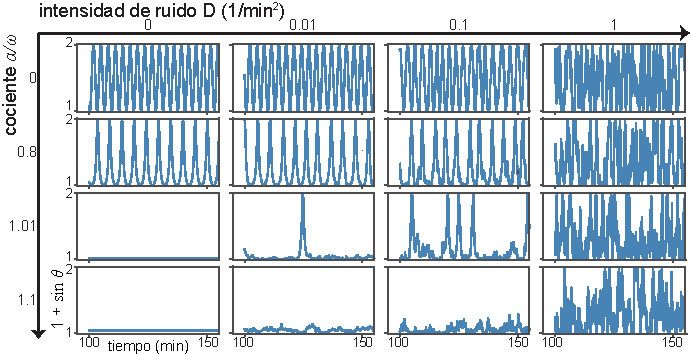
\includegraphics[width=1\columnwidth]{figures/chapter6/C6_traces.pdf} 
    \caption{\textbf{Actividad pulsátil en el régimen excitable del modelo de fase con bifurcación de ciclo infinito y ruido blanco gaussiano aditivo.} Series temporales que representan la dinámica de la fase gobernada por la ecuación \ref{C6_eq:adler_white_noise}, en donde el observable es \ref{C5_eq:seno_fase}. De arriba hacia abajo, la primera fila representa el caso oscilatorio uniforme. La segunda fila representa el caso de oscilaciones no uniformes, y las dos filas restantes son casos excitables. Las series temporales fueron obtenidas a partir de simulaciones descriptas en el apéndice \ref{C6_ap:traces}, donde la frecuencia del caso oscilatorio uniforme $\omega = 18\pi/28 \; \text{min}$, la frecuencia de sampleo $dt$ fue de $10^{-4}$, la frecuencia de adquisición $d$ fue de $10$, el total de tiempo de la simulación $T$ fue de $1000$ minutos. Las condiciones iniciales fueron sampleadas de una distribución uniforme $U(0,2\pi)$. Las series temporales fueron graficadas desde los $100$ minutos para evitar visualizar efectos transitorios.}
    \label{C6_fig:traces} 
\end{figure}


\marginpar{espectro de consenso}
En definitiva, el ruido promueve la aparición de pulsos en el régimen excitable, y la tasa de pulsado aumenta, al menos cualitativamente, conforme a la intensidad del ruido. A diferencia del régimen oscilatorio, en este régimen no hay una estructura temporal periódica subyacente que los ordene. 

Para estudiar estructuras dinámicas en series temporales pulsátiles, es común utilizar observables basados en el espectro de potencias de Fourier, ya que tienen un significado intuitivo inmediato y son fácilmente medibles en series temporales sintéticas \cite{Gammaitoni1998}. Definimos el espectro de consenso de las series temporales $s(t)$ como \cite{Ditzinger1994}
\begin{equation}
    \langle S_k \rangle = \frac{1}{N} \sum_{i=1}^N |A_k|^2,
    \label{C6_eq:espectro_consenso}
\end{equation}
donde $A_k$ es el espectro de amplitud de Fourier definido según \ref{C2_eq:amplitud_fourier}, y $N$ es la cantidad de series temporales consideradas. 


En la figura \ref{C6_fig:SR}A graficamos el espectro de consenso de series temporales adquiridas en el régimen excitable. Para valores bajos de intensidad de ruido, el espectro de consenso muestra un pequeño máximo en frecuencias bajas. La altura del máximo del espectro y su frecuencia fundamental aumentan con la intensidad del ruido $D$. Tras un valor umbral de intensidad de ruido, la altura del pico del espectro y la frecuencia fundamental comienzan a disminuir. Finalmente, para un $D$ suficientemente grande, la frecuencia fundamental se desplaza a cero, efecto característico de las dinámicas completamente dominadas por el ruido. Este comportamiento del espectro de consenso en función del ruido sugiere la presencia de una dinámica pulsátil coherente estimulada por el ruido, en donde la coherencia está optimizada  en valores intermedios de $D$. 


\marginpar{factor de calidad}
Para formalizar esta interpretación, podemos usar del factor de calidad, un parámetro adimensional que cuantifica el rendimiento de un oscilador o resonador. Formalmente, definimos el factor de calidad $\beta$ como \cite{Ditzinger1994}
\begin{equation}
    \beta = \omega_0 \frac{\langle S_0 \rangle}{\Delta  \omega_0},
    \label{C6_eq:QF}
\end{equation}
donde $\langle S_0 \rangle$ es la amplitud del espectro de consenso de la señal $s(t)$ en su frecuencia fundamental $\omega_0$. $\Delta  \omega_0$ es una medida del ancho del espectro de consenso en su frecuencia fundamental, definido como el ancho del espectro cuando su altura es $\frac{\langle S_0 \rangle}{\sqrt{e}}$. Con esta definición, el factor de calidad es grande cuando el ancho del espectro de consenso es pequeño, es decir, cuando adquirimos señales \emph{puras} del sistema.  El factor $\omega_0$ de esta definición determina que el factor de calidad será mayor a frecuencias mayores, frecuencias que se alejan del ruido blanco. 


En la figura  \ref{C6_fig:SR}B podemos observar el factor de calidad correspondiente a los datos de la figura \ref{C6_fig:SR}A. Observamos que $\beta$ aumenta conforme a la intensidad del ruido, manifestando una dinámica cada vez más coherente. Luego de alcanzar un máximo, la curva del factor de calidad decrece, retratando que el ruido destruye gradualmente el movimiento coherente. El máximo revela la existencia de un ruido óptimo que produce la dinámica más coherente dentro del régimen excitable. Este efecto es propio de sistemas de resonancia estocástica. \marginpar{resonancia estocástica sin excitación}


 \begin{figure}
    \centering
    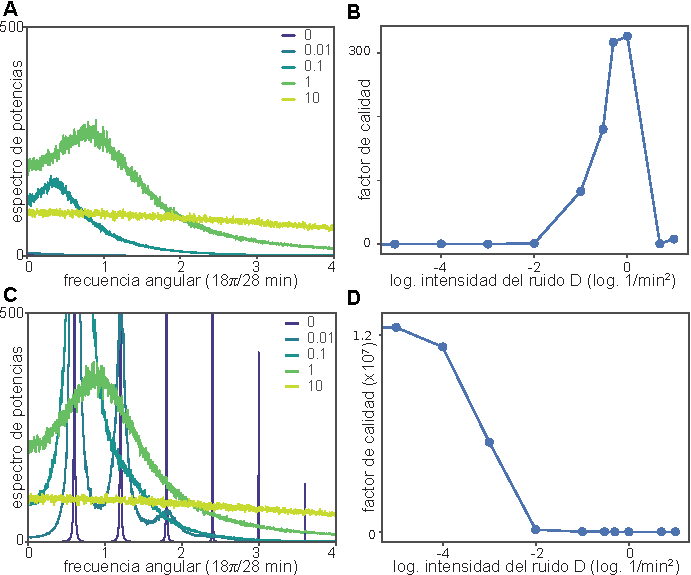
\includegraphics[width=1\columnwidth]{figures/chapter6/C6_SR.pdf} 
    \caption{\textbf{Resonancia estocástica en el régimen excitable del modelo de fase con bifurcación infinita y ruido blanco aditivo.} (A) Espectro de consenso de $N=500$ series temporales simuladas para el caso excitable del modelo de fase de bifurcación de ciclo infinito con ruido blanco gaussiano aditivo (ecuación \ref{C6_eq:espectro_consenso}, apéndice \ref{C6_ap:traces}).$\omega = 18\pi/28 \; \text{min}$ y $\ddelta = 1.1$. (B) Factor de calidad en función de la intensidad del ruido, calculado a partir de los datos de A (ecuación \ref{C6_eq:QF}). (C) Espectro de consenso de $N=500$ series temporales simuladas para el caso oscilatorio no uniforme del modelo de fase de bifurcación de ciclo infinito con ruido blanco gaussiano aditivo. $\omega = 18\pi/28 \; \text{min}$ y $\ddelta = 0.8$. (D) Factor de calidad en función de la intensidad del ruido, calculado a partir de los datos de C. (A-D) La frecuencia de sampleo $dt$ fue de $10^{-4}$, la frecuencia de adquisición $d$ fue de $10$, el total de tiempo de la simulación $T$ fue de $1000$ minutos, y las condiciones iniciales fueron sampleadas de una distribución uniforme $U(0,2\pi)$.(A,C) La intensidad del ruido está indicada en escala de colores. }
    \label{C6_fig:SR}
\end{figure}

%VER
Por completitud, en la figura \ref{C6_fig:SR}C,D mostramos el espectro de consenso y el factor de calidad para el caso de oscilaciones no uniformes. Para valores bajos de ruido, donde domina el comportamiento determinista, el espectro de frecuencias consiste en una frecuencia fundamental bien definida, y frecuencias secundarias que reflejan la no uniformidad de la señal. A medida que aumenta la intensidad del ruido, el pico del espectro se va ensanchando y corriendo hacia frecuencias fundamentales más grandes y el factor de calidad decrece. Esto indica que el ruido destruye gradualmente el movimiento coherente determinista. Si la intensidad del ruido es lo suficientemente grande, el espectro de Fourier indica que el movimiento está completamente dominado por el ruido. 


En definitiva, el régimen excitable del sistema \ref{C6_eq:adler_white_noise} tiene una estructura de pulsado, en donde el ruido regula la coherencia de la actividad pulsátil en el régimen excitable, y la desordena en el régimen oscilatorio. La resonancia estocástica que observamos en el régimen excitable del modelo estudiado refuerza la idea que motiva este capítulo, donde hipotetizamos que perturbando de manera sistemática al sistema en el régimen excitable podemos conseguir oscilaciones intermitentes- transiciones entre períodos oscilatorios, silencios y pulsos aislados-. Por otro lado, comienza a ser interesante también la idea de evaluar si las oscilaciones intermitentes que observamos pueden ser descriptas como oscilaciones desordenadas. 


Otra característica que creemos relevante de la dinámica que queremos describir es la duración de pulsos. Los resultados que obtuvimos en el capítulo anterior para el modelo determinista muestran que la duración de pulsos depende de la frecuencia del homogéneo y de la amplitud de modulación, y es sensible a las perturbaciones que dan lugar a la actividad pulsátil en este régimen. Sin embargo, en el modelo de fase con bifurcación de ciclo infinito y ruido blanco aditivo la duración de pulsos no está caracterizada sistemáticamente. Continuando nuestra caracterización de este modelo, nos proponemos obtener una expresión para este observable, para poder estudiar su dependencia de los distintos parámetros de la descripción teórica.


\section{La duración de pulsos depende de la intensidad del ruido}
\sectionmark{La duración de pulsos depende de ...}
\label{C6_sec:duracion}


Queremos obtener una expresión analítica de la duración de pulsos del sistema dinámico \ref{C6_eq:adler_white_noise}. Para el régimen excitable, en \ref{C5_sec:T_exc} definimos un pulso cuando el sistema sobrepasa el punto fijo inestable \xxi y realiza una excursión hacia el punto fijo estable siguiente \xxe, siendo su duración $T_{exc}$ el tiempo que tarda el sistema en llegar \emph{al entorno de} \xxe, habiendo partido \emph{del entorno de} \xxi. La versión estocástica \ref{C6_eq:adler_white_noise} tiene la ventaja de que no es necesario posicionarse en el entorno de los puntos fijos, pues es el ruido quien eventualmente perturbará al sistema y generará una excursión o pulso. Sin embargo, el carácter estocástico del sistema añade cierta complejidad al cálculo de este observable.

Para una sola trayectoria del sistema en el régimen excitable, podemos pensar a la duración de un pulso como el tiempo que tarda el sistema en alcanzar el punto fijo estable \xxe, dado que el comenzó en el punto fijo inestable \xxi y durante ese tiempo no volvió al punto fijo inestable \xxi. Como distintas posibles trayectorias del sistema pueden tener pulsos con distinta duración, la duración de pulsos es una variable aleatoria y su distribución de probabilidad asociada determina la posibilidad de que se den los diferentes valores. Para nuestros objetivos, es suficiente estudiar cómo depende la duración de pulsos media de la intensidad del ruido. Para obtener una expresión analítica de la duración de pulsos media, es útil trabajar con el tiempo de primer pasaje condicional medio. 


\marginpar{tiempo de\\primer pasaje\\condicional medio}
En el contexto de este problema, el tiempo de primer pasaje medio para un sistema estocástico es el tiempo medio que tarda el sistema en alcanzar un determinado umbral por primera vez, dada su condición inicial \cite{Redner2001}. De esta definición, el tiempo de primer pasaje condicional medio es el tiempo medio que tarda el sistema en alcanzar un determinado umbral de llegada por primera vez dada su condición inicial, y dado que no cruzó un umbral prohibido en el trayecto.  

\marginpar{duración de\\pulsos media}
En el régimen excitable, definimos \textbf{el tiempo de primer pasaje condicional medio} \tplus(\xx) como el tiempo que le toma al sistema alcanzar el punto fijo estable \xxe por primera vez, dado que salió de \xx y nunca pasó por el punto fijo inestable \xxi. Con esta idea, definimos la \textbf{duración de pulsos media} $T_\xi$ en el excitable como el tiempo medio que tarda el sistema en llegar a al punto fijo estable \xxe, habiendo salido pero nunca vuelto a pasar por el punto fijo inestable \xxi, es decir,
\begin{align}
    T_\xi = \lim_{\xx \rightarrow \xxi}\tplus(\xx).
    \label{C6_eq:Txi_def}
\end{align}.

Para el caso oscilatorio, es intuitivo pensar que la duración de pulsos media es el tiempo medio que tarda el sistema en alcanzar $\xx_0+2\pi$, habiendo salido y no vuelto a $\xx_0$. Este problema también es un problema de tiempo de primer pasaje condicional, y es trivial extender la definición \ref{C6_eq:Txi_def} a este régimen reemplazando $\xxi \rightarrow \xx_0$ y $\xxe \rightarrow \xx_0+2\pi$. Por simplicidad, trabajaremos con la notación \ref{C6_eq:Txi_def} más amigable para el régimen excitable, y luego haremos los reemplazos correspondientes para estudiar la duración de pulsos media en el régimen oscilatorio. 

Para obtener una expresión analítica de la duración de pulsos media, comenzaremos por obtener una expresión para el tiempo de primer pasaje condicional medio. Primero buscaremos obtener una ecuación diferencial para esta variable, y luego indagaremos sobre su solución. Finalmente, tomaremos el límite \ref{C6_eq:Txi_def} para obtener la duración de pulsos.

\subsection{Ecuación diferencial para el tiempo de primer pasaje condicional medio}
\sectionmark{Tiempo de primer pasaje condicional medio}

Como nos interesa solamente el tiempo de primer pasaje condicional \emph{medio}, utilizaremos el formalismo de Laplace, es decir, la versión integrada de la ecuación de tiempo de primer pasaje condicional \cite{Redner2001}.

\marginpar{probabilidad condicional \epsplus(\xx)}
Primero definimos \epsplus(\xx) como la probabilidad de que el sistema llegue al punto fijo estable \xxe sin pasar por el punto fijo inestable \xxi, habiendo salido de \xx contenido en $[ \,\xxi,\xxe ]\,$. Podemos calcular a \epsplus(\xx) como
\begin{equation}
    \epsplus(\xx) = \sum_{p_{+}} P_{p_{+}}(\xx),
    \label{C6_eq:mFPT_eps_def}
\end{equation}
donde $P_{p_{+}}(\xx)$ es la probabilidad de una única trayectoria $p_{+}$ que comienza en \xx llegue a \xxe evitando \xxi. 

Para encontrar una expresión analítica de \epsplus(\xx), comenzaremos por trabajar con un problema de \textit{random walk} unidimensional no simétrico a primeros vecinos en el intervalo finito $[\xxi,\xxe ]$, y más adelante tomaremos el límite al continuo. 


Un problema de \textit{random walk} es un proceso aleatorio que describe una trayectoria que consiste en una sucesión de pasos aleatorios. Entonces, imaginemos que el sistema se encuentra en \xx. Si consideramos el problema unidimensional y a primeros vecinos, el sistema puede moverse solamente un paso a la izquierda o un paso a la derecha en un instante de tiempo. Entonces, en un instante de tiempo posterior, el sistema se encontrará en \xx+\deltax con una probabilidad $q(\xx)$, y en \xx-\deltax con una probabilidad $1-q(\xx)$, donde la función $q(\xx)$ determina la asimetría del \textit{random walk}. Esta propiedad es fácil de ver en el límite de \textit{random walk} simétrico, donde $q(\xx) = \frac{1}{2}$ y el sistema tiene la misma probabilidad de estar un paso adelante \xx+\deltax y un paso atrás \xx-\deltax. En cambio, para otros valores de $q(\xx)$, el sistema tendrá una probabilidad distinta de estar un paso adelante que un paso atrás. Como agregado, proponemos la posibilidad de que $q(\xx)$ dependa de la localización del sistema \xx, pero que sea independiente del tiempo. 

Con esta interpretación, podemos escribir la suma \ref{C6_eq:mFPT_eps_def} sobre todas las trayectorias restringidas como la suma sobre todos los caminos posibles empezando luego del primer paso,
\begin{align}
    \epsplus(\xx) &= \sum_{p_{+}} ( q(\xx) P_{p_{+}}(\xx + \deltax) + (1-q(\xx)) P_{p_{+}}(\xx - \deltax)) \\
    & = q(\xx) \epsplus(\xx+\deltax) +  (1-q(\xx)) \epsplus(\xx - \deltax) 
    \label{C6_eq:mFPT_eps_S1}.
\end{align}
Si asumimos que \deltax es pequeño comparado con \xx, podemos desarrollar en series la expresión \ref{C6_eq:mFPT_eps_S1}, y
\begin{align}
    \epsplus(\xx) = & q(\xx) \big[  \epsplus(\xx) + \epsplus'(\xx) \; \deltax + \epsplus''(\xx) \; \frac{\deltax^2}{2} \big] + \nonumber \\  & (1-q(\xx)) \big[  \epsplus(\xx) - \epsplus'(\xx) \; \deltax + \epsplus''(\xx) \; \frac{\deltax^2}{2} \big].
\end{align}
Luego,
\begin{align}
    \epsplus(\xx) &=  \epsplus(\xx) + (2q(\xx)-1) \epsplus'(\xx) \; \deltax + \epsplus''(\xx) \; \frac{\deltax^2}{2} \\
    0 &=  (2q(\xx)-1) \epsplus'(\xx) \; \deltax + \epsplus''(\xx) \; \frac{\deltax^2}{2}. \label{C6_eq:mFPT_eps_S2}
\end{align}
La expresión \ref{C6_eq:mFPT_eps_S2} no es más que una ecuación diferencial para \epsplus(\xx). Antes de toma el límite al continuo, dividimos a la expresión \ref{C6_eq:mFPT_eps_S2} por el incremento temporal $\delta t$,
\begin{align}
     0 =  (2q(\xx)-1) \epsplus'(\xx) \; \frac{\deltax}{\delta t} + \epsplus''(\xx) \; \frac{\deltax^2}{2 \delta t}. 
     \label{C6_eq:mFPT_eps_S3}
\end{align}
Para tomar el límite al continuo, donde $\delta t \rightarrow   0 $ y $\deltax \rightarrow 0$, es necesario definir
\begin{equation}
    v(\xx) = (2q(\xx)-1) \frac{\deltax}{\delta t} \qquad D = \frac{\deltax^2}{2 \delta t} \qquad \text{con} \; \delta t \rightarrow   0 \; \text{y} \; \deltax \rightarrow 0 .
    \label{C6_eq:mFPT_eps_def_vD}
\end{equation}
Si incorporamos esta definición a la expresión \ref{C6_eq:mFPT_eps_S3},
\begin{align}
     0 &=  v(\xx) \epsplus'(\xx) + D \epsplus''(\xx) .
     \label{C6_eq:mFPT_eps_S4}
\end{align}
Luego, conseguimos una ecuación diferencial que describe \epsplus(\xx), en donde aún desconocemos $v(\xx)$ y $D$. Para escribir una expresión para estos coeficientes, definamos $P(\xx,t)$ como la probabilidad de estar en \xx a tiempo $t$. Siguiendo un razonamiento análogo al anterior, podemos escribir a la probabilidad de estar en \xx a tiempo $t+\delta t$ operando sobre sus contribuciones: (i) la probabilidad de haber hecho un paso hacia adelante desde \xx - \deltax en el instante t, sumado a (ii) la probabilidad de haber hecho un paso hacia atrás desde \xx + \deltax en el instante t, más (iii) la probabilidad de estar en \xx en el instante t y no realizar ningún movimiento , menos (iv) la probabilidad de originalmente estar en \xx a tiempo t y moverse para adelante y (v) para atrás, tal que 
\begin{align}
    P(\xx,t + \delta t ) &=  q(\xx - \deltax) P(\xx-\deltax,t) + (1-q(\xx + \deltax)) P(\xx+\deltax,t) \nonumber \\ +& P(\xx,t) - q(\xx) P(\xx,t) - (1-q(\xx)) P(\xx,t).
    \label{C6_eq:mFPT_eps_S5}
\end{align}
Otra vez, podemos asumir que \deltax es pequeño comparado con \xx y expandir a la expresión \ref{C6_eq:mFPT_eps_S5} en una serie de potencias a segundo orden, 
\begin{align}
    & P( \xx,t + \delta t) - P(\xx,t) = \nonumber \\
    & \big[ q(\xx) - q'(\xx)\deltax + q''(\xx) \frac{\deltax^2}{2}  \big] \big[ P(\xx,t) - \partial_\xx P(\xx,t) \deltax + \partial_{\xx \xx} P(\xx,t) \frac{\deltax^2}{2}  \big] \nonumber \\ & + \big[ 1 - q(\xx) - q'(\xx)\deltax - q''(\xx) \frac{\deltax^2}{2}  \big] \big[ P(\xx,t) + \partial_\xx P(\xx,t) \deltax + \partial_{\xx \xx} P(\xx,t) \frac{\deltax^2}{2}  \big] \nonumber \\ & - P(\xx,t) .
\end{align}
Luego, 
\begin{align}
    & P( \xx,t + \delta t) - P(\xx,t) = \nonumber \\
    & P(\xx,t) \big[ q(\xx) - q'(\xx)\deltax + q''(\xx) \frac{\deltax^2}{2} + 1 - q(\xx) - q'(\xx)\deltax - q''(\xx) \frac{\deltax^2}{2} -1\big] \nonumber \\ & + \partial_\xx P(\xx,t) \; \deltax \; \big[ - q(\xx) + q'(\xx)\deltax - q''(\xx) \frac{\deltax^2}{2} + 1 - q(\xx) - q'(\xx)\deltax - q''(\xx) \frac{\deltax^2}{2}\big] \nonumber \\ &+ \partial_{\xx \xx} P(\xx,t) \;  \frac{\deltax^2}{2} \; \big[  q(\xx) - q'(\xx)\deltax + q''(\xx) \frac{\deltax^2}{2} +  1 - q(\xx) - q'(\xx)\deltax - q''(\xx) \frac{\deltax^2}{2} \big] .
\end{align}
Si simplificamos la expresión que conseguimos, 
\begin{align}
     & P( \xx,t + \delta t) - P(\xx,t) = \nonumber \\
     & - 2 q'(\xx) \; \deltax \; P(\xx,t) + \big[ 1- 2 q(\xx) - q''(\xx) \deltax^2 \big] \; \deltax \; \partial_\xx P(\xx,t) \nonumber \\ & +\big[ 1-2 q'(\xx) \deltax \big] \frac{\deltax^2}{2}\partial_{\xx \xx} P(\xx,t)  .
     \label{C6_eq:mFPT_eps_S6}
\end{align}
Como estamos considerando términos hasta el segundo orden, despreciamos los proporcionales a $\deltax^3$. Si luego dividimos \ref{C6_eq:mFPT_eps_S6} por el incremento temporal $\delta t$,
\begin{align}
    & \frac{P( \xx,t + \delta t) - P(\xx,t)}{\delta t}  = \nonumber \\ & - 2 q'(\xx) \frac{\deltax}{\delta t} P(\xx,t) + \big[ 1- 2 q(\xx) \big] \frac{\deltax}{\delta t} \partial_\xx P(\xx,t) +  \frac{\deltax^2}{2 \delta t}\partial_{\xx \xx} P(\xx,t).
    \label{C6_eq:mFPT_eps_S7}
\end{align}
Teniendo en cuenta que 
\begin{align}
    \partial_\xx\big( (1-2q(\xx)) \frac{\deltax}{\delta t} \big) = - 2 q'(\xx) \frac{\deltax}{\delta t},
\end{align}
podemos reescribir la expresión \ref{C6_eq:mFPT_eps_S7} como 
\begin{align}
    \frac{P(\xx,t) - P(\xx,t) }{\delta t} &= - \partial_\xx \big[ (1-2q(\xx)) \frac{\deltax}{\delta t} P(\xx,t) \big] + \frac{\deltax^2}{2 \delta t}\partial_{\xx \xx} P(\xx,t).
\end{align}
Finalmente, tomamos el límite al continuo y redefinimos según \ref{C6_eq:mFPT_eps_def_vD}, 
\begin{align}
   \partial_t P(\xx,t) &= - \partial_\xx \big[ v(\xx) P(\xx,t) \big] + D \partial_{\xx \xx} P(\xx,t).
   \label{C6_eq:mFPT_eps_S8}
\end{align}
La ecuación \ref{C6_eq:mFPT_eps_S8} se trata de la ecuación de \emph{Fokker Planck} para un proceso homogeneo, donde el \emph{drift} $v(\xx)$ y la \emph{difusión} $D$ son independientes del tiempo. El proceso estocástico que describe la solución de la ecuación \ref{C6_eq:mFPT_eps_S8} es equivalente al que describe la ecuación diferencial estocástica de Itô \cite{Gardiner}
\begin{equation}
    \partial_t  \theta(t) =  v(\xx) + \sqrt{2D} \xi_w(t).
\end{equation}
Comparando esta ecuación diferencial con \ref{C6_eq:adler_white_noise}, es fácil determinar que 
\begin{align}
    v(\xx) = \omega + \alpha \sin{(\xx)}  \label{C6_eq:mFPT_eps_def_vD_solved}
\end{align}
y $D$ es la intensidad del ruido. Una vez escrita una expresión para los coeficientes $v(\xx)$ y $D$, podemos finalmente escribir la ecuación diferencial que describe \epsplus(\xx) a partir de reemplazar a estos coeficientes en \ref{C6_eq:mFPT_eps_S4}
\begin{align}
     0 &=  (\omega + \alpha \sin{(\xx)}) \epsplus'(\xx) + D \epsplus''(\xx) .
     \label{C6_eq:mFPT_eps_eq_res}
\end{align}
Recordemos que la \epsplus(\xx) es la probabilidad de que el sistema llegue al punto fijo estable \xxe sin pasar por el punto fijo inestable \xxi, habiendo salido de $ \xx  \in [ \,\xxi,\xxe ]\,$. Luego, por definición, la probabilidad de que el sistema llegue al punto fijo estable \xxe sin pasar por el punto fijo inestable \xxi habiendo salido de \xxi es nula. Además, la probabilidad de que el sistema llegue al punto fijo estable \xxe sin pasar por el punto fijo inestable \xxi habiendo salido de \xxe es uno. Estos dos casos triviales constituyen las condiciones de contorno de \ref{C6_eq:mFPT_eps_eq_res}
\begin{align}
    \epsplus(\xxi) = 0 \qquad \epsplus(\xxe) = 1.
    \label{C6_eq:mFPT_eps_cdc}
\end{align}
% VER comentar sobre el análogo electrostático?


Ahora, estamos en condiciones de intentar derivar una ecuación diferencial para el tiempo de primer pasaje condicional medio \tplus(\xx). Formalmente, definimos el tiempo de primer pasaje condicional medio \tplus(\xx) como el tiempo medio que tarda el sistema en llegar al punto fijo estable \xxe sin haber pasado por el punto fijo inestable \xxi, habiendo salido de \xx contenido en $[ \,\xxi,\xxe ]\,$. Si pensamos que $t_{p_{+}}(\xx)$ es el tiempo que tarda una trayectoria posible $p_{+}$ en realizar el recorrido y $P_{p_{+}}$ la probabilidad de que cada una de esas posibles trayectorias ocurra,
\begin{align}
    \tplus(\xx) &= \frac{\sum_{p_{+}}p_{+}(\xx) t_{p_{+}}(\xx)}{\sum_{p_{+}}p_{+}(\xx)}\\
    & = \frac{\sum_{p_{+}}p_{+}(\xx) t_{p_{+}}(\xx)}{\epsplus(\xx)},
\end{align}
en donde para calcular el valor medio dividimos sobre la suma de probabilidades de las trayectorias posibles, y luego usamos la definición \ref{C6_eq:mFPT_eps_def}. Luego,
\begin{align}
    \tplus(\xx) \epsplus(\xx)  &= \sum_{p_{+}}p_{+}(\xx) t_{p_{+}}(\xx) 
    \label{C6_eq:mFPT_tplus_def}
\end{align}
Con un razonamiento análogo al realizado para obtener la ecuación \ref{C6_eq:mFPT_eps_S1}, 
\begin{align}
   & \tplus(\xx) \epsplus(\xx) = \sum_{p_{+}} \Big[ q(\xx)  p_{+}(\xx + \deltax ) \big( t_{p_{+}}(\xx + \deltax) + \delta t \big)  \nonumber \\ & + \big( 1 - q(\xx) \big)  p_{+}(\xx - \deltax ) \big( t_{p_{+}}(\xx - \deltax) + \delta t \big)\Big] \\
   & =  q(\xx) \sum_{p_{+}} p_{+}(\xx + \deltax ) t_{p_{+}}(\xx + \deltax) + q(\xx) \sum_{p_{+}} p_{+}(\xx + \deltax ) \delta t  \nonumber \\ & + \big( 1 - q(\xx) \big) \sum_{p_{+}}p_{+}(\xx - \deltax ) t_{p_{+}}(\xx - \deltax) +  \big( 1 - q(\xx) \big) \sum_{p_{+}}p_{+}(\xx - \deltax ) \delta t .
\end{align}
Usamos las definiciones \ref{C6_eq:mFPT_tplus_def} y \ref{C6_eq:mFPT_eps_def} para reemplazar las sumatorias
\begin{align}
   \tplus(\xx) \epsplus(\xx) & = q(\xx) \tplus(\xx + \deltax) \epsplus(\xx + \deltax) + q(\xx) \epsplus(\xx + \deltax) \delta t \nonumber \\ & + \big( 1 - q(\xx) \big) \tplus(\xx - \deltax) \epsplus(\xx - \deltax) +  \big( 1 - q(\xx) \big) \epsplus(\xx - \deltax) \delta t.
   \label{C6_eq:mFPT_tplus_S1}
\end{align}
Para simplificar la lectura, definimos  $\epstplus(\xx) =  \tplus(\xx) \epsplus(\xx)$, y \ref{C6_eq:mFPT_tplus_S1} queda escrita como
\begin{align}
   \epstplus(\xx) & = q(\xx) \epstplus(\xx + \deltax) + q(\xx) \epsplus(\xx + \deltax) \delta t \nonumber \\ & + \big( 1 - q(\xx) \big) \epstplus(\xx - \deltax) +  \big( 1 - q(\xx) \big) \epsplus(\xx - \deltax) \delta t.
   \label{C6_eq:mFPT_tplus_S2}
\end{align}
Si nuevamente consideramos $\deltax \ll \xx$, podemos realizar el desarrollo en series de \ref{C6_eq:mFPT_tplus_S2} hasta segundo orden en \deltax. Para construir este desarrollo en series, comencemos por expresar los primeros órdenes de \epstplus(\xx) y \epsplus(\xx) 
\begin{align}
    \epstplus(\xx \pm \deltax) & = \epstplus(\xx) \pm \epstplus'(\xx) \deltax + \epstplus''(\xx) \frac{\deltax^2}{2} \\
    \epsplus(\xx \pm \deltax) & = \epsplus(\xx) \pm \epsplus'(\xx) \deltax + \epsplus''(\xx) \frac{\deltax^2}{2}.
\end{align}
Si reemplazamos estas cantidades en \ref{C6_eq:mFPT_tplus_S2},
\begin{align}
       & \epstplus(\xx) = q(\xx) \Bigg[  \epstplus(\xx) + \epstplus'(\xx) \deltax + \epstplus''(\xx) \frac{\deltax^2}{2} \Bigg] + q(\xx) \delta t \Bigg[  \epsplus(\xx) + \epsplus'(\xx) \deltax + \epsplus''(\xx) \frac{\deltax^2}{2}\Bigg] \nonumber \\ & +  \big( 1 - q(\xx) \big) \Bigg[  \epstplus(\xx) - \epstplus'(\xx) \deltax + \epstplus''(\xx) \frac{\deltax^2}{2} \Bigg] \nonumber \\ & + \big( 1 - q(\xx) \big) \delta t \Bigg[  \epsplus(\xx) - \epsplus'(\xx) \deltax + \epsplus''(\xx) \frac{\deltax^2}{2}\Bigg] .
\end{align}
Simplificando,
\begin{align}
        \epstplus(\xx) & = \epstplus(\xx) + \big(2 q(\xx) -1 \big) \; \deltax \;  \epstplus'(\xx)  +  \frac{\deltax^2}{2}  \epstplus''(\xx) \nonumber \\ & + \delta t \; \epsplus(\xx)  + \big(2 q(\xx) -1 \big) \; \deltax \; \delta t \;  \epsplus'(\xx) +  \frac{\deltax^2}{2} \; \delta t \; \epsplus''(\xx) .
        \label{C6_eq:mFPT_tplus_S3}
\end{align}
Si dividimos toda la expresión \ref{C6_eq:mFPT_tplus_S3} por el incremento temporal $\delta t$, y luego tomamos el límite al continuo  $\delta t \rightarrow   0 $ y $\deltax \rightarrow 0$, 
\begin{align}
       0 &= v(\xx) \epstplus'(\xx)  + D \epstplus''(\xx) + \epsplus(\xx)\\
       -\epsplus(\xx) &= v(\xx) \epstplus'(\xx)  + D \epstplus''(\xx),
\end{align}
en donde utilizamos el resultado \ref{C6_eq:mFPT_eps_S4} y las definiciones de \ref{C6_eq:mFPT_eps_def_vD}.
Finalmente, logramos obtener una ecuación diferencial para el producto $\epsplus(\xx) = \epsplus(\xx) \tplus(\xx)$, y
\begin{align}
       - \epsplus(\xx) &= v(\xx) (\epsplus(\xx) \tplus(\xx)))'  + D (\epsplus(\xx) \tplus(\xx)))''  \\
     - \epsplus(\xx) &= (\omega + \alpha \sin{(\xx)}) (\epsplus(\xx) \tplus(\xx)))'  + D (\epsplus(\xx) \tplus(\xx)))'' ,
       \label{C6_eq:mFPT_tplus_eq_res}
\end{align}
donde en la última ecuación utilizamos la expresión  \ref{C6_eq:mFPT_eps_def_vD_solved}.

De \ref{C6_eq:mFPT_eps_cdc} sabemos que \epsplus(\xx) se anula en \xxi, por ende el producto \epsplus(\xx) \tplus(\xx) también lo hará. Por otro lado, recordemos que \tplus(\xx) era el tiempo medio que tarda el sistema en llegar al punto fijo estable \xxe sin haber pasado por el punto fijo inestable \xxi, habiendo salido de \xx. Luego, es trivial que \tplus(\xx) se anula en \xxe. Con estas dos características, tenemos las condiciones de contorno correspondientes a la ecuación diferencial \ref{C6_eq:mFPT_tplus_eq_res}
\begin{align}
    \epsplus(\xxe) \tplus(\xxe) = 0 \qquad \epsplus(\xxi) \tplus(\xxi) = 0 .
    \label{C6_eq:mFPT_tplus_eq_cdc}
\end{align}

Resolviendo las ecuaciones \ref{C6_eq:mFPT_tplus_eq_res} y \ref{C6_eq:mFPT_tplus_eq_cdc}, junto con \ref{C6_eq:mFPT_eps_eq_res} y \ref{C6_eq:mFPT_eps_cdc} podremos encontrar una expresión analítica para el tiempo de primer pasaje condicional medio \tplus(\xx). 

%no entiendo si poner o no el tema de el FPT no condicional

\subsection{Expresión analítica del tiempo de primer pasaje condicional medio}

Como primer paso, buscaremos obtener una expresión analítica para la probabilidad condicional \epsplus(\xx) resolviendo el sistema de ecuaciones \ref{C6_eq:mFPT_eps_S4} y \ref{C6_eq:mFPT_eps_cdc}. De \ref{C6_eq:mFPT_eps_S4},
\begin{align}
     \frac{\epsplus''(\xx)}{\epsplus'(\xx)} = - \frac{v(\xx)}{D}.
\end{align}
Si definimos $f(\xx) = \epsplus'(\xx)$, $\frac{\partial f}{\partial\xx}(\xx) = \epsplus''(\xx) $ y
\begin{align}
     \frac{f(\xx)}{df} = - \frac{v(\xx)}{D} d\xx.
     \label{C6_eq:mFPT_eps_R1}
\end{align}
Integramos a ambos lados de la ecuación \ref{C6_eq:mFPT_eps_R1}, 
\begin{align}
     \ln{(f(\xx))} = - \frac{V(\xx)}{D} + C,
\end{align}
donde $V(\xx)$ es la primitiva de $v(\xx)$, y en $C$ absorbimos todas las constantes de integración. Luego,
\begin{align}
     f(\xx) &= \frac{1}{N} e^{- \frac{V(\xx)}{D}} \\
     \epsplus'(\xx) & =\frac{1}{N} e^{- \frac{V(\xx)}{D}}, 
     \label{C6_eq:mFPT_eps_R2}
\end{align}
donde $\frac{1}{N}$ es una constante positiva. Logramos obtener la solución homogénea de $\epsplus'(\xx)$. Para obtener una expresión para \epsplus(\xx), hay que integrar \ref{C6_eq:mFPT_eps_R2}. En esta integración, elegimos los límites de integración de manera de cumplir la condición de contorno $\epsplus(\xxi) = 0 $ de \ref{C6_eq:mFPT_eps_cdc} y
\begin{align}
     \epsplus(\xx) & = \frac{1}{N} \int_{\xxi}^\xx e^{- \frac{V(\xx)}{D}} .
\end{align}
Para determinar $N$ utilizaremos la otra condición de contorno de \ref{C6_eq:mFPT_eps_cdc}
\begin{align}
     \epsplus(\xxe) & = \frac{1}{N} \int_{\xxi}^{\xxe} e^{- \frac{V(\xx)}{D}} = 1. 
\end{align}
Luego,
\begin{align}
      N &= \int_{\xxi}^{\xxe} e^{- \frac{V(\xx)}{D}} . 
\end{align}
Con este resultado, logramos obtener una expresión para \epsplus(\xx) 
\begin{align}
     \epsplus(\xx) & = \frac{\int_{\xxi}^\xx e^{- \frac{V(\xx)}{D}}}{\int_{\xxi}^{\xxe} e^{- \frac{V(\xx)}{D}}} \\
     \epsplus(\xx) & = \frac{\int_{\xxi}^\xx e^{- \frac{\omega \xx - \alpha \cos{(\xx)}}{D}}}{\int_{\xxi}^{\xxe} e^{- \frac{\omega \xx - \alpha \cos{(\xx)}}{D}}},
     \label{C6_eq:mFPT_eps_res}
\end{align}
en donde reemplazamos $V(\xx) = \omega \xx - \alpha \cos{(\xx)}$.


Para analizar el resultado \ref{C6_eq:mFPT_eps_res}, es útil tomar el límite del oscilador uniforme, donde $\alpha = 0$, la dinámica determinista del oscilador uniforme consiste en oscilaciones a velocidad angular constante $\omega$, y no hay puntos fijos. Entonces, sin pérdida de generalidad podemos considerar
\begin{align}
    v(\xx) = \omega \qquad 
    \xxi = 0 \qquad \xxe = 2 \pi
    \label{C6_eq:mFPT_uniforme}
\end{align}
Con estos valores, la probabilidad \epsplus(\xx) es
\begin{align}
     \epsplus(\xx) & = \frac{\int_{0}^\xx e^{- \frac{\omega \xx}{D}}}{\int_{0}^{2\pi} e^{- \frac{\omega \xx}{D}}}
      = \frac{\frac{-D}{\omega} \big[e^{- \frac{\omega \xx}{D}} - 1\big]}{\frac{-D}{\omega} \big[e^{- \frac{\omega 2\pi}{D}} - 1\big]} = \frac{ 1 - e^{- \frac{\omega \xx}{D}}}{1- e^{- \frac{\omega 2\pi}{D}}}.
\end{align}
Esta expresión coincide con lo reportado previamente \cite{Redner2001}. Esta expresión es creciente en \xx, lo que indica que cuanto más cerca del punto fijo estable, mayor probabilidad de llegar hasta él sin cruzar antes el punto fijo inestable. Este resultado es intuitivo, pues el sistema necesita recorrer menos distancia, lo que conduce a una mayor probabilidad de éxito. Además, a mayor frecuencia del uniforme y a menor intensidad del ruido, ese crecimiento es más abrupto. Es decir, cuanto más domine la dinámica determinista por sobre el ruido, mayor probabilidad de éxito para recorrer la misma trayectoria. 


Para verificar el resultado \ref{C6_eq:mFPT_eps_res}, contamos en simulaciones computacionales cuántas trayectorias llegaban satisfactoriamente a \xxe para el sistema cuya dinámica estaba gobernada por la ecuación \ref{C6_eq:adler_white_noise} e inicialmente se encontraba en \xx. Descartamos todas las mediciones realizadas sobre las trayectorias que atravesaban \xxi y normalizamos las cuentas por el número total de simulaciones realizadas (ver apéndice \ref{C6_ap:traces}). En la figura \ref{C6_fig:mFPT_eps} graficamos \epsplus(\xx) en función de la condición inicial \xx. Para todos los casos, la expresión \ref{C6_eq:mFPT_eps_res} que obtuvimos coincide con las mediciones computacionales que realizamos.


En la figura \ref{C6_fig:mFPT_eps}A observamos que para valores pequeños de ruido, la función \epsplus(\xx) es mayoritariamente uno, menos en un entorno pequeño del punto fijo inestable, que es cero. Para valores chicos de ruido, siempre que el sistema empiece fuera del punto fijo inestable, inevitablemente termina en el punto fijo inestable y no vuelve al punto fijo estable. A medida que aumenta la intensidad del ruido, \epsplus(\xx) se va suavizando y pareciéndose cada vez más a la recta de pendiente unidad, característica de problemas de \textit{random walk} simétricos, lo que sugiere que en ese régimen la dinámica está gobernada por el ruido. 


A medida que aumentamos el cociente adimensional \ddelta para valores de intensidad del ruido y frecuencia del uniforme fijos, la localización de los puntos fijos en el régimen excitable cambia según \ref{C5_eq:PF_def}. En la figura \ref{C6_fig:mFPT_eps}B es llamativo que la probabilidad condicional \epsplus(\xx) en el caso régimen oscilatorio uniforme, en el oscilatorio no uniforme y en el excitable tiene la misma forma. 

Finalmente, en la figura  \ref{C6_fig:mFPT_eps}C podemos ver que la concavidad de la probabilidad condicional \epsplus(\xx) es levemente más abrupta conforme aumenta la frecuencia del uniforme $\omega$.  Cuando aumenta la frecuencia del uniforme, aumenta la velocidad que el sistema puede tomar dentro del intervalo $[\xxi,\xxe]$. Luego, el ruido tiene menos tiempo (o probabilidad) para perturbar al sistema hacia el punto fijo inestable. 


\begin{figure}
    \centering
    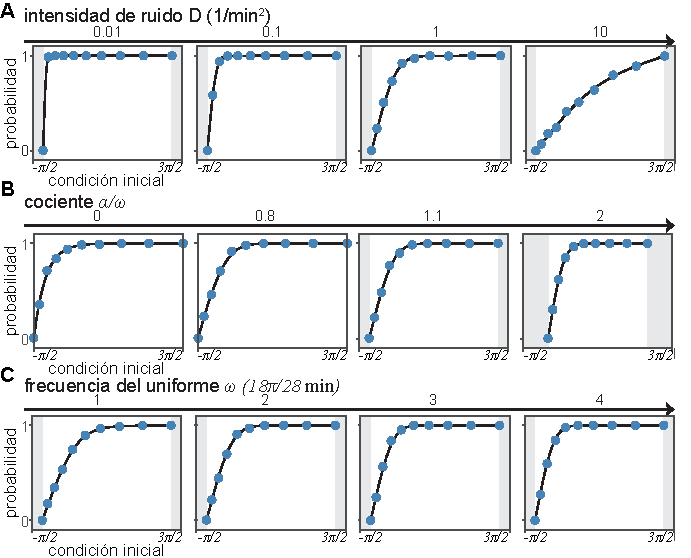
\includegraphics[width=1\columnwidth]{figures/chapter6/C6_eps_plus.pdf} 
    \caption{\textbf{Probabilidad condicional \epsplus(\xx) de llegar a \xxe sin pasar por \xxi en función de la condición inicial \xx.} (A) Probabilidad condicional \epsplus(\xx) en función de su condición inicial \xx para distintos valores de intensidad de ruido, indicados arriba. $\omega = 18\pi/28$, y $\ddelta = 1.1$. (B) Probabilidad condicional \epsplus(\xx) en función de su condición inicial \xx para distintos valores del cociente adimensional \ddelta, indicados arriba. $\omega = 18\pi/28$, y $D = 1$. (C) Probabilidad condicional \epsplus(\xx) en función de su condición inicial \xx para distintos valores de frecuencia del uniforme, indicados arriba. $\ddelta = 1.1$ y $D=1$. (A-C) Los puntos azules indican los resultados de los cálculos numéricos, la línea negra es el resultado de la expresión analítica \ref{C6_eq:mFPT_eps_res}, y los bordes de la región gris indican el punto fijo inestable (izquierda) o estable (derecha) si corresponde. Las simulaciones numéricas fueron $N=500$, con un paso $dt = 10^{-5}$ y una frecuencia de adquisición de $d=1$.}
    \label{C6_fig:mFPT_eps}
\end{figure}



Una vez que encontramos la solución a \ref{C6_eq:mFPT_eps_S4}, estamos en condiciones de comenzar a trabajar con \ref{C6_eq:mFPT_tplus_eq_res} para obtener la expresión analítica del tiempo de primer pasaje condicional medio $\tplus(\xx)$. Como \ref{C6_eq:mFPT_tplus_eq_res} es una ecuación diferencial para la derivada de este producto $ \epstplus(\xx) = \epsplus(\xx) \tplus(\xx) $,  primero obtendremos una expresión para la derivada de este producto, luego integraremos la solución e impondremos las condiciones de contorno \ref{C6_eq:mFPT_tplus_eq_cdc}, para finalmente obtener la expresión analítica de  $\tplus(\xx)$.


Utilizaremos el método de variación constante para dar con una expresión de \Depstplus(\xx). Como primer paso, queremos determinar la solución homogénea $\DepstplusH(\xx)$ de \ref{C6_eq:mFPT_tplus_eq_res}, y
\begin{align}
    0 &= v(\xx) \DepstplusH(\xx)  + D \DDepstplusH(\xx)\\
    \frac{\DDepstplusH(\xx)}{\DepstplusH(\xx)} &= - \frac{v(\xx)}{D}, 
\end{align}
y
\begin{align}
   \DepstplusH(\xx) & = K  e^{- \frac{V(\xx)}{D}},
\end{align}
donde $V(\xx)$ es la primitiva de $v(\xx)$ y $K$ es una constante positiva.
Luego, permitimos $K \rightarrow   K(\xx)$ tal que $\Depstplus(\xx) = K(\xx) e^{- \frac{V(\xx)}{D}}$, y buscamos hallar la solución particular de \ref{C6_eq:mFPT_tplus_eq_res}
\begin{align}
    - \epsplus(\xx) &= v(\xx) \Depstplus(\xx) + D \DDepstplus(\xx)\\
    - \epsplus(\xx) &= v(\xx) K(\xx) e^{- \frac{V(\xx)}{D}}  \nonumber \\
    & + D K'(\xx)e^{- \frac{V(\xx)}{D}} - D K(\xx) \frac{v(\xx)}{D} e^{- \frac{V(\xx)}{D}} \\
    - \epsplus(\xx) &=  D K'(\xx)e^{- \frac{V(\xx)}{D}} .
\end{align}
Entonces
\begin{align}
         K'(\xx) = - \frac{\epsplus(\xx)}{D} e^{ \frac{V(\xx)}{D}} .
\end{align}
Para encontrar $K(\xx)$ tomamos un límite de integración arbitrario $\xx_{0}$
\begin{align}
         K(\xx) - K_0 = \frac{-1}{D} \int_{\xx_0}^\xx d\xx' \epsplus(\xx') e^{ \frac{V(\xx')}{D}},
\end{align}
donde $K_0 = K(\xx_0)$. Con este resultado, 
\begin{align}
    \Depstplus(\xx) = \frac{-e^{- \frac{V(\xx)}{D}}}{D} \int_{\xx_0}^\xx d\xx' \epsplus(\xx') e^{ \frac{V(\xx')}{D}} + K_0 \; e^{- \frac{V(\xx)}{D}} .
\end{align}
Luego, 
\begin{align}
   \epstplus(\xx) = \int_{\xx_1}^{\xx} d\xx'  \frac{- e^{- \frac{V(\xx')}{D}} }{D} \int_{\xx_0}^{\xx'} d \xx'' \epsplus(\xx'') e^{ \frac{V(\xx'')}{D}} + K_0 \int_{\xx_1}^{\xx} d\xx'  e^{- \frac{V(\xx')}{D}}  .
\end{align}


Si elegimos $\xx_1 = \xxi$, la integral $\int_{\xx_1 = \xxi}^{\xx} d\xx'  e^{- \frac{V(\xx')}{D}} = N \epsplus(\xx)$, y además se cumple una de las condiciones de contorno \ref{C6_eq:mFPT_tplus_eq_cdc} donde $\epstplus(\xxi) = 0$. Luego,
\begin{align}
   \epstplus(\xx) = \int_{\xx_1}^{\xx} d\xx'  \frac{- e^{- \frac{V(\xx')}{D}} }{D} \int_{\xx_0}^{\xx'} d \xx'' \epsplus(\xx'') e^{ \frac{V(\xx'')}{D}} + N \epsplus(\xx) K_0 .
\end{align}
Si definimos $I_0(\xx) =  \frac{-1}{D} \int_{\xx_0}^\xx d \xx' \epsplus(\xx') e^{ \frac{V(\xx')}{D}}$, 
\begin{align}
   \epstplus(\xx) &= \int_{\xxi}^{\xx} d\xx'  e^{- \frac{V(\xx')}{D}}  I_0(\xx')+  N \; \epsplus(\xx) \; K_0 .
   \label{C6_eq:mFPT_tplus_R1}
\end{align}
Si aprovechamos que $ e^{- \frac{V(\xx)}{D}} = N \epsplus(\xx)'$, podemos reescribir la expresión \ref{C6_eq:mFPT_tplus_R1} usando partes para descomponer el término de la integral,
\begin{align}
   \epstplus(\xx) &= I_0(\xx') N \epsplus(\xx') \Bigg]_{\xxi}^{\xx} - \int_{\xxi}^{\xx} d\xx' N \epsplus(\xx') \Big(\frac{-1}{D} \epsplus(\xx') e^{ \frac{V(\xx')}{D}} \Big) +  N \epsplus(\xx) K_0 \\
            &= I_0(\xx) N \epsplus(\xx) - I_0(\xxi) N \epsplus(\xxi) + \frac{N}{D} \int_{\xxi}^{\xx} d\xx'  \epsplus^2(\xx') e^{ \frac{V(\xx')}{D}} +  N \epsplus(\xx) K_0 \\
            &= I_0(\xx) N \epsplus(\xx) + \frac{N}{D} \int_{\xxi}^{\xx} d\xx'  \epsplus^2(\xx') e^{ \frac{V(\xx')}{D}} +  N \epsplus(\xx) K_0 ,
\end{align}
donde en la última igualdad usamos $\epsplus(\xxi) = 0$. Finalmente, 
\begin{align}
   \epstplus(\xx) &= \big(I_0(\xx)+K_0\big) N \epsplus(\xx) + \frac{N}{D} \int_{\xxi}^{\xx} d\xx'  \epsplus^2(\xx') e^{ \frac{V(\xx')}{D}}. 
\end{align}
Ahora podemos determinar las constantes $K_0$ y $\theta_0$ con las condiciones de contorno.
\begin{align}
   \epstplus(\xxe) &= \big(I_0(\xxe)+K_0\big) N \epsplus(\xxe) + \frac{N}{D} \int_{\xxi}^{\xxe} d\xx'  \epsplus^2(\xx') e^{ \frac{V(\xx')}{D}} = 0\\
   0&=\big(I_0(\xxe)+K_0\big) + \frac{1}{D} \int_{\xxi}^{\xxe} d\xx'  \epsplus^2(\xx') e^{ \frac{V(\xx')}{D}} \\
   0&=\frac{-1}{D} \int_{\xx_0}^{\xxe} d \xx' \epsplus(\xx') e^{ \frac{V(\xx')}{D}} +K_0 + \frac{1}{D} \int_{\xxi}^{\xxe} d\xx'  \epsplus^2(\xx') e^{ \frac{V(\xx')}{D}} \\
   K_0 &= \frac{1}{D} \Big( \int_{\xx_0}^{\xxe} d \xx' \epsplus(\xx') e^{ \frac{V(\xx')}{D}} - \int_{\xxi}^{\xxe} d\xx'  \epsplus^2(\xx') e^{ \frac{V(\xx')}{D}}\Big)
\end{align}
Si elegimos $\xx_0 = \xxe$,
\begin{align}
   K_0 &= \frac{-1}{D} \int_{\xxi}^{\xxe} d\xx'  \epsplus^2(\xx') e^{ \frac{V(\xx')}{D}}.
\end{align}
Para terminar, ya tenemos nuestro resultado 
\begin{align}
   \epstplus(\xx) &= \frac{-N}{D} \epsplus(\xx) \Big(  \int_{\xx_e}^\xx d \xx' \epsplus(\xx') e^{ \frac{V(\xx')}{D}} +  \int_{\xxi}^{\xxe} d\xx'  \epsplus^2(\xx') e^{ \frac{V(\xx')}{D}} \nonumber \\ & - \frac{1}{\epsplus(\xx)} \int_{\xxi}^{\xx} d\xx'  \epsplus^2(\xx') e^{ \frac{V(\xx')}{D}} \Big)\\
     \epstplus(\xx) &= \frac{N}{D} \epsplus(\xx) \Big(  \int_\xx^{\xx_e} d \xx' \epsplus(\xx') e^{ \frac{V(\xx')}{D}} -  \int_{\xxi}^{\xxe} d\xx'  \epsplus^2(\xx') e^{ \frac{V(\xx')}{D}} \nonumber \\ & + \frac{1}{\epsplus(\xx)} \int_{\xxi}^{\xx} d\xx'  \epsplus^2(\xx') e^{ \frac{V(\xx')}{D}} \Big)
\end{align}
Finalmente, logramos tener la expresión para el tiempo de primer pasaje condicional medio
\begin{align}
     \tplus(\xx)&= \frac{N}{D} \Big(  \int_\xx^{\xx_e} d \xx' \epsplus(\xx') e^{ \frac{V(\xx')}{D}} -  \int_{\xxi}^{\xxe} d\xx'  \epsplus^2(\xx') e^{ \frac{V(\xx')}{D}} + \frac{1}{\epsplus(\xx)} \int_{\xxi}^{\xx} d\xx'  \epsplus^2(\xx') e^{ \frac{V(\xx')}{D}} \Big) \label{C6_eq:mFPT_tplus_res}
\end{align}

Si tomamos el límite del oscilador uniforme \ref{C6_eq:mFPT_uniforme}, el tiempo de primer pasaje condicional medio es 
\begin{align}
     \tplus(\xx)& = \frac{2 \pi \left(e^{\frac{2 \pi \omega}{D}}+1\right) \left(e^{\frac{\omega \xx}{D}}-1\right)-\xx\left(e^{\frac{2 \pi\omega}{D}}-1\right) \left(e^{\frac{\omega \xx}{D}}+1\right)}{\omega \left(e^{\frac{2 \pi \omega}{D}}-1\right) \left(e^{\frac{\omega \xx}{D}}-1\right)},
     \label{C6_eq:mFPT_tplus_res_alpha_cero} 
\end{align}
expresión que coincide con resultados previamente reportados \cite{Redner2001}. De esta expresión, es interesante notar que cuando la intensidad de ruido tiende a cero, \ref{C6_eq:mFPT_tplus_res_alpha_cero} tiende a $\frac{2\pi - \xx}{\omega}$, y cuando la condición inicial es $0$, el tiempo coincide con el período del oscilador uniforme. Luego, el segundo término de \ref{C6_eq:mFPT_tplus_res_alpha_cero} es la corrección correspondiente a empezar en cualquier lugar \xx del círculo. 


Para corroborar \ref{C6_eq:mFPT_tplus_res}, medimos en simulaciones computacionales cuánto tiempo tardaba el sistema cuya dinámica estaba gobernada por la ecuación \ref{C6_eq:adler_white_noise} e inicialmente se encontraba en \xx en llegar a \xxe. Descartamos todas las mediciones realizadas sobre las trayectorias que atravesaban \xxi (ver apéndice \ref{C6_ap:traces}). En la figura \ref{C6_fig:mFPT_tplus} observamos que nuestra expresión coincide con las simulaciones. Observamos, además, que en todos los casos el tiempo de primer pasaje medio condicional decrece conforme aumenta la condición inicial. Además, si la condición inicial tiende a ser el punto fijo inestable, el tiempo es finito y depende de los parámetros del modelo. 


En \ref{C6_fig:mFPT_tplus}A podemos observar que el ruido tiende a disminuir el tiempo de primer pasaje condicional medio. En \ref{C6_fig:mFPT_tplus}B observamos que el cociente adimensional \ddelta tiene el mismo efecto, pues la velocidad que el sistema puede tener en el intervalo $[\xxi,\xxe]$ aumenta con el cociente \ddelta, así como la distancia entre la condición inicial \xx y el punto fijo estable. De manera similar, un aumento de la frecuencia del uniforme conduce a velocidades mayores que el sistema puede tomar en el intervalo $[\xxi,\xxe]$, que termina aplanando la curva del tiempo de primer pasaje medio condicional (figura \ref{C6_fig:mFPT_tplus}C). 


\begin{figure}
    \centering
    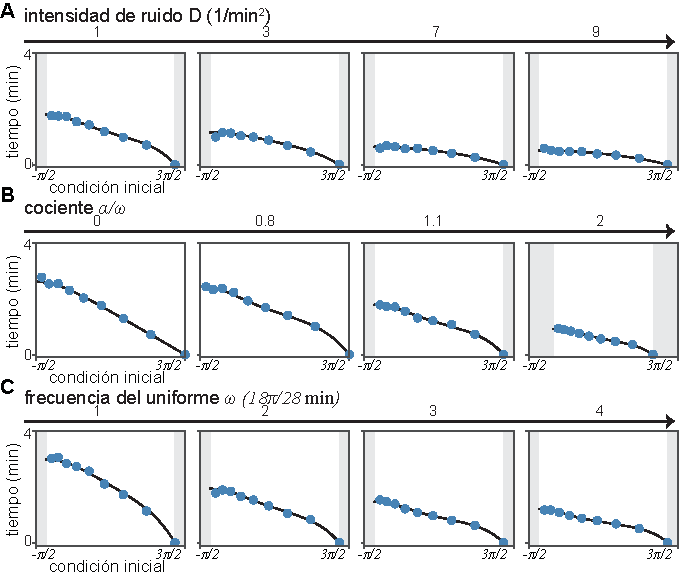
\includegraphics[width=1\columnwidth]{figures/chapter6/C6_t_plus.pdf} 
    \caption{\textbf{Tiempo medio \tplus(\xx) para llegar al punto fijo estable \xxe sin pasar por el punto fijo inestable \xxi en función de la condición inicial \xx.} (A) Tiempo medio \tplus(\xx) en función de su condición inicial \xx para distintos valores de intensidad de ruido. $\omega = 18\pi/28$, y $\ddelta = 1.1$. (B) Tiempo medio \tplus(\xx) en función de su condición inicial \xx para distintos valores del cociente adimensional \ddelta. $\omega = 18\pi/28$, y $D = 1$. (C) Tiempo medio \tplus(\xx) en función de su condición inicial \xx para  distintos valores de frecuencia del uniforme. $\ddelta = 1.1$ y $D=1$. (A-C) Los puntos azules indican los resultados de los cálculos numéricos, la línea negra indica el resultado de la expresión analítica \ref{C6_eq:mFPT_tplus_res}, y los bordes de la región gris indican el punto fijo inestable (izquierda) o estable (derecha) si corresponde. Las simulaciones numéricas fueron $N=500$, con un paso $dt = 10^{-5}$ y una frecuencia de adquisición de $d=1$.}
    \label{C6_fig:mFPT_tplus}
\end{figure}

\subsection{Expresión analítica para la duración de pulsos media}
\sectionmark{Duración de pulsos media}

En la sección anterior observamos que el límite \ref{C6_eq:Txi_def} que define la duración de pulsos media del sistema \ref{C6_eq:adler_white_noise} es finito y depende de los parámetros del modelo. En esta sección queremos obtener una expresión analítica para la duración de pulsos media $T_\xi$, que definimos como el tiempo medio que tarda el sistema en llegar a \xxe, habiendo salido pero nunca vuelto a pasar por \xxi.


Comenzamos por reescribir la ecuación \ref{C6_eq:mFPT_tplus_res} para tener una expresión con límites de integración más sencillos,
\begin{align}
     \tplus(\xx)&= \frac{N}{D} \Big(  \int_\xx^{\xx_e} d \xx' \epsplus(\xx') e^{ \frac{V(\xx')}{D}} -  \int_{\xxi}^{\xxe} d\xx'  \epsplus^2(\xx') e^{ \frac{V(\xx')}{D}} \nonumber \\ & + \frac{1}{\epsplus(\xx)} \int_{\xxi}^{\xx} d\xx'  \epsplus^2(\xx') e^{ \frac{V(\xx')}{D}} \Big) \\
     &= \frac{N}{D} \Big[  \int_\xx^{\xx_e} d \xx' \epsplus(\xx') e^{ \frac{V(\xx')}{D}} \big(1 - \epsplus(\xx') \big)+ \nonumber \\ & \big( \frac{1}{\epsplus(\xx)} -1 \big) \int_{\xxi}^{\xx} d\xx'  \epsplus^2(\xx') e^{ \frac{V(\xx')}{D}} \Big]. \label{C6_eq:Txi_tplus_terminos}
\end{align}

Tenemos una expresión que es la suma de dos integrales. Comenzaremos por trabajar con el primer término 
\begin{align}
     \lim_{\xx \rightarrow   \xxi }&\frac{N}{D}  \int_\xx^{\xxe} d \xx' \epsplus(\xx') e^{ \frac{V(\xx')}{D}} \big(1 - \epsplus(\xx') \big) \\
     &= \frac{N}{D} \int_{\xxi}^{\xxe} d \xx' \epsplus(\xx') e^{ \frac{V(\xx')}{D}} \big(1 - \epsplus(\xx') \big).
     \label{C6_eq:Txi_LI1}
\end{align}


Luego, detengámonos en el segundo término de \ref{C6_eq:Txi_tplus_terminos}. Es fácil ver que la integral de este término tiende a cero cuando $\xx \rightarrow \xxi $, pues el límite de integración superior tiende al límite de integración inferior. Esto mismo ocurre con \epsplus(\xx). Según su expresión analítica \ref{C6_eq:mFPT_eps_res}, $\epsplus(\xx) \rightarrow 0$ cuando $\xx \rightarrow \xxi $. Esta indeterminación hacen que este límite no sea fácil de calcular. Luego, para determinar el límite del segundo término, es necesario salvar la indeterminación 
\begin{align}
      \lim_{\xx \rightarrow   \xxi }& \frac{1}{\epsplus(\xx)}  \int_{\xxi}^{\xx} d\xx'  \epsplus^2(\xx') e^{ \frac{V(\xx')}{D}}.
     \label{C6_eq:Txi_LI2_S1}
\end{align}
A partir de \ref{C6_eq:mFPT_eps_res}, podemos determinar que 
\begin{align}
     \epsplus'(\xx) & = \frac{e^{- \frac{V(\xx)}{D}}}{N},
\end{align}
y en particular 
\begin{align}
     \epsplus'(\xxi) & = \frac{e^{- \frac{V(\xxi)}{D}}}{N} = \frac{e^{- \frac{\omega \xxi - \alpha \cos{(\xxi)}}{D}}}{N} \neq 0.
\end{align}
Luego, como $\epsplus'(\xxi)$ no se anula ni en \xxi ni en su entorno, podemos usar la regla de L'Hospital para salvar la indeterminación \ref{C6_eq:Txi_LI2_S1}
\begin{align}
     & \lim_{\xx \rightarrow   \xxi } \frac{1}{\epsplus(\xx)}  \int_{\xxi}^{\xx} d\xx'  \epsplus^2(\xx') e^{ \frac{V(\xx')}{D}}\\
     & = \lim_{\xx \rightarrow   \xxi } \frac{1}{\frac{e^{- \frac{V(\xx)}{D}}}{N}}  \; \epsplus^2(\xx) e^{ \frac{V(\xx)}{D}} \\
     & = \frac{1}{\frac{e^{- \frac{V(\xxi)}{D}}}{N}}  \; \epsplus^2(\xxi) e^{ \frac{V(\xxi)}{D}} \\
     & = \frac{1}{\frac{e^{- \frac{V(\xxi)}{D}}}{N}}  \times 0. 
     \label{C6_eq:Txi_LI2_S2}
\end{align}
Mientras que el primer término de \ref{C6_eq:Txi_LI2_S2} es distinto de cero, su segundo término tiende a cero. Para corroborar este límite, estudiamos el comportamiento de \ref{C6_eq:Txi_LI2_S1} en un entorno de \xxi (figura \ref{C6_fig:Txi_LI2_S2}).

\begin{figure}
    \centering
    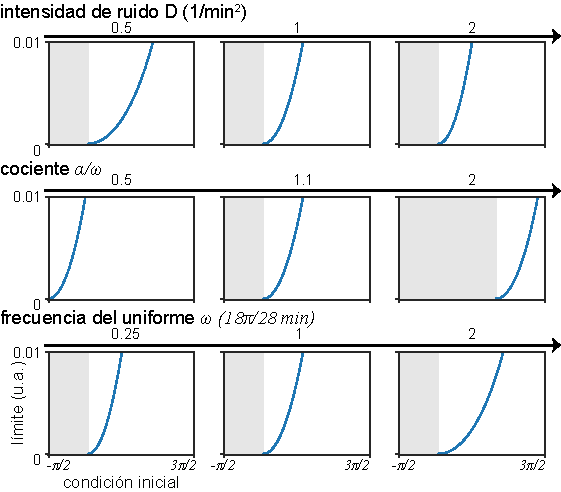
\includegraphics[width=1\columnwidth]{figures/chapter6/C6_limite_int_2.pdf} 
    \caption{\textbf{Comportamiento de \ref{C6_eq:Txi_LI1} cerca del punto fijo inestable \xxi}. Comportamiento de \ref{C6_eq:Txi_LI1} cerca del punto fijo inestable \xxi para distintos valores de la intensidad del ruido $D$, cociente adimensional $\alpha/\omega$ y frecuencia del homogéneo $\omega$ indicados. $\omega = \frac{2\pi}{7 \text{min}}$, $\ddelta = 1.1$ , y $\D = 1 \frac{1}{\text{min}^2}$, a excepción de que se especifique otro valor. Los bordes de la región gris indican el punto fijo inestable si corresponde}
    \label{C6_fig:Txi_LI2_S2}
\end{figure}

Con estos resultados, obtuvimos una expresión analítica para la duración de pulsos
\begin{align}
     T_\xi = \frac{\int_{\xxi}^{\xxe} d \xx' \epsplus(\xx') e^{ \frac{V(\xx')}{D}} \big(1 - \epsplus(\xx') \big)}{D\; \int_{\xxi}^{\xxe} e^{- \frac{V(\xx)}{D}}},
     \label{C6_eq:Txi}
\end{align}
en donde la principal contribución se corresponde al limite \ref{C6_eq:Txi_LI1}.

Para verificar la expresión \ref{C6_eq:Txi}, medimos en simulaciones computacionales cuánto tiempo tardaba el sistema cuya dinámica estaba gobernada por la ecuación \ref{C6_eq:adler_white_noise} e inicialmente se encontraba en \xxi en llegar a \xxe. Descartamos todas las mediciones realizadas sobre las trayectorias que atravesaban \xxi luego del instante inicial (ver apéndice \ref{C6_ap:traces}). En la figura \ref{C6_fig:duration} observamos que nuestra expresión coincide con las simulaciones. 


\begin{figure}
    \centering
    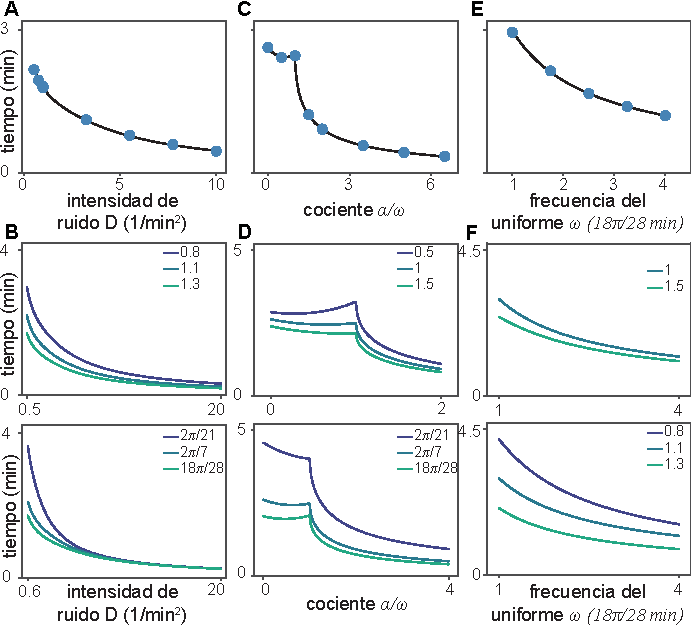
\includegraphics[width=1\columnwidth]{figures/chapter6/C6_duration.pdf} 
    \caption{\textbf{Duración de pulsos $T_\xi$ del modelo de fase con bifurcación de ciclo infinito y ruido blanco gaussiano aditivo.} (A,B) Duración de pulsos $T_\xi$ en función de la intensidad de ruido $D$. En B el cociente adimensional \ddelta (arriba) y la frecuencia del uniforme (abajo, en $1/\text{min}$) se encuentran codificados en escala de colores. (C,D) Duración de pulsos $T_\xi$ en función de el cociente adimensional \ddelta. En D la intensidad de ruido (arriba, en $1/\text{min}^2$) y la frecuencia del uniforme (abajo, en $1/\text{min}$) se encuentran codificados en escala de colores. (E,F) Duración de pulsos $T_\xi$ en función de la frecuencia del uniforme $\omega$. En F la intensidad de ruido (arriba, en $1/\text{min}^2$) y la frecuencia del uniforme (abajo, en $1/\text{min}$) se encuentran codificados en escala de colores (A-F). $\omega = \frac{18\pi}{28 \text{min}}$, $\ddelta = 1.1$ , y $D = 1 \frac{1}{\text{min}^2}$, a excepción de que se especifique otro valor. (A,C,E)  Los puntos azules indican los resultados de los cálculos numéricos, y la línea negra indica el resultado de la expresión analítica \ref{C6_eq:Txi}. Las simulaciones numéricas fueron $N=10^6$, con un paso $dt = 10^{-5}$ y una frecuencia de adquisición de $d=1$.}
    \label{C6_fig:duration}
\end{figure}


En el panel A de la figura \ref{C6_fig:duration} observamos que la duración de pulsos disminuye conforme aumenta el ruido. Además, la escala temporal del comportamiento disminuye conforme aumenta el cociente \ddelta, y la frecuencia del uniforme $\omega$ (figura \ref{C6_fig:duration}B). Es también interesante que para valores altos de intensidad de ruido, las curvas convergen a una duración límite finita. 

En el panel C de la figura \ref{C6_fig:duration} observamos la duración de pulsos en función de \ddelta. Podemos observar una discontinuidad en el comportamiento en $\ddelta = 1$, donde ocurre la bifuración de \textit{saddle node} de ciclo infinito en el modelo determinista del capítulo \ref{ch5}. Para el caso oscilatorio donde $\ddelta < 1$, si la duración de pulsos es creciente o decreciente con \ddelta depende de los parámetros $D$ y $\omega$ (figura \ref{C6_fig:duration}D). En particular, la duración de pulsos en la bifurcación aumenta con el ruido. Es razonable hipotetizar que para valores muy pequeños de ruido la duración de pulsos en el régimen oscilatorio tienda a comportarse según \ref{C5_eq:T_osc}, y en el excitable según \ref{C5_eq:T_exc}. En particular, podemos pensar que con elecciones correctas de $\omega$ y $D$, podemos conseguir duraciones de pulsos similares si variamos $\alpha$ cerca de la bifurcación. En el régimen excitable donde $\ddelta > 1$, la duración de pulsos siempre decrece conforme aumenta \ddelta. 

Observamos que para frecuencias del uniforme cada vez más altas, la duración de pulsos disminuye (figuras \ref{C6_fig:duration} E,F).  


En resumen, observamos que la duración de pulsos del modelo estocástico depende de los parámetros del modelo de una manera no trivial. Observamos analíticamente y con simulaciones computacionales que la duración de pulsos depende del ruido tanto en el caso excitable como en el oscilatorio. Esta dependencia es uniforme, y menores duraciones se consiguen con mayores valores de intensidad de ruido. También hayamos que para valores de ruido y frecuencia del uniforme fijos, variar $\alpha$ en un entorno del valor de bifurcación puede eventualmente conducir a oscilaciones en el régimen oscilatorio, y actividad pulsátil en el régimen excitable, con duraciones de pulso similares cerca de la bifurcación. En principio, esta caracterización es compatible con que haya un conjunto de parámetros que den origen a una duración de pulsos como en la que observamos en los experimentos. En lo próximo, evaluamos concretamente la posibilidad de que el modelo teórico propuesto pueda reproducir la estadística de nuestras mediciones experimentales, para luego calibrarlo y entender qué características de las oscilaciones intermitentes de actividad de ERK es capaz de reproducir. 


\section{Capacidades y limitaciones para describir las oscilaciones intermitentes de actividad de ERK}
\sectionmark{Capacidades para describir oscilaciones intermitentes}


En las secciones anteriores observamos que el modelo de fase con bifurcación de ciclo infinito y ruido blanco gaussiano con una amplitud de modulación mayor a la frecuencia del uniforme puede dar lugar a actividad pulsátil. Esta actividad pulsátil es producto de perturbaciones que genera el ruido en el régimen excitable. Estudiamos que, en estas condiciones, los valores de ruido regulan la coherencia de esta actividad pulsátil. Por otro lado, cuando la amplitud de modulación es menor que la frecuencia del uniforme, el ruido desordena las oscilaciones. Estas características convierten a este modelo teórico en un candidato interesante para describir las oscilaciones intermitentes. Sin embargo, observamos que las propiedades dinámicas de la fase, como la duración de pulsos, dependen de los parámetros del modelo de una manera no trivial.  

En este marco, en esta sección nos preguntamos qué capacidad tiene el modelo de fase con bifurcación de ciclo infinito y ruido blanco gaussiano de reproducir las oscilaciones intermitentes de la dinámica de actividad de ERK en ESCs. Comenzamos por analizar la posibilidad que el modelo teórico ajuste a observables calculados sobre los datos experimentales. Elegimos observables simples y que resumen muchas de las principales características de la dinámica de activación de ERK en ESCs, y comparamos su estadística calculada sobre el modelo teórico con la de nuestros datos experimentales. De esta manera, buscamos entender si las propiedades dinámicas de la descripción teórica son compatibles con nuestras observaciones experimentales. En segundo lugar, diseñamos un protocolo para ajustar de manera sistemática los observables calculados sobre el modelo teórico a los calculados sobre los experimentos. A partir de esta calibración, evaluamos qué magnitudes dinámicas que describen las oscilaciones intermitentes en nuestras observaciones experimentales puede reproducir el modelo.


\subsection{Observables para comparar el modelo con los experimentos}

Para comparar el modelo con los datos experimentales, decidimos enfocarnos en la estadística de la duración de pulsos (ecuación \ref{C2_eq:duracion_de_pulsos}, figura \ref{C6_fig:observables_experimentales}A), el intervalo de interpulsado (ecuación \ref{C2_eq:IPI}, figura \ref{C6_fig:observables_experimentales}B), y la tasa de pulsado -definida como el número de pulsos dividido por la duración de la serie temporal- (sección \ref{C3_ssec:analisis_cuantitativo}, figura \ref{C6_fig:observables_experimentales}C). 

A nuestro entender, la duración de pulsos es la principal característica dinámica de los pulsos individuales. El intervalo de interpulsado es una medida cuantitativa simple que informa acerca de cómo están ordenados los pulsos en la serie temporal. Finalmente, la tasa de pulsado es una medida sencilla de la actividad pulsátil en las series temporales experimentales. Esperamos, además, que el ajuste simultáneo de la duración de pulsos y la tasa de pulsado conduzca al ajuste del tiempo medio que las células estuvieron pulsando (figura \ref{C2_fig:actividad}, ecuación \ref{C2_eq:actividad}). 

\begin{figure}
    \centering
    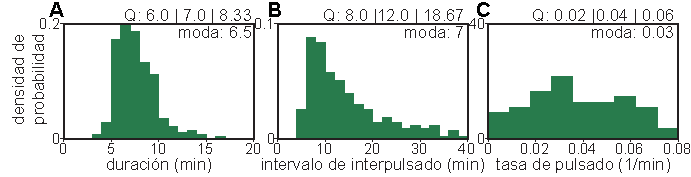
\includegraphics[width=1\columnwidth]{figures/chapter6/C6_experimental_stats.pdf} 
    \caption{\textbf{Observables representativos de los datos experimentales.} (A) Distribución de la duración de pulsos. Las unidades del eje $y$ son (1/min). (B) Distribución de intervalo de interpulsado. Las unidades del eje $y$ son (1/min). (C) Distribución de tasa de pulsado. Las unidades del eje $y$ son min. (A-C) Los datos experimentales fueron adquiridos en serum + LIF (capítulo \ref{ch2}). N = 69 células, $n_1$ = 289 pulsos, $n_2$ = 225 pares de pulsos. Los cuartiles (Q) 25, 50 y 75 y la moda se indican en la parte superior de cada gráfico. Fueron excluidos de los histogramas 9 (en B) y 7 (en C) puntos mayores que el límite del eje x.}
    \label{C6_fig:observables_experimentales}
\end{figure}

Para comparar el modelo con los experimentos, es necesario calcular la estadística de estos observables en el modelo teórico, por ejemplo midiendo estas cantidades en series temporales sintéticas de la variable angular \xx en función del tiempo $t$. 

\marginpar{duración de pulsos}
Retomando las definiciones de la sección \ref{C6_sec:duracion}, en el régimen excitable de \ref{C6_eq:adler_white_noise} definimos un pulso cuando el sistema sobrepasa el punto fijo inestable \xxi y realiza una excursión hacia el punto fijo estable siguiente \xxe sin volver a \xxi. En estas circunstancias, el inicio del pulso es el punto fijo inestable \xxi, y su final es el punto fijo estable siguiente \xxe.  Para el caso oscilatorio, definimos un pulso cuando el sistema alcanza $\xx_0+2\pi$, habiendo partido y no vuelto a $\xx_0$.  Es decir, el inicio del pulso es un punto arbitrario $\xx_0$, y el final del pulso es $\xx_0+2\pi$. Con estas definiciones en mente, la \textbf{duración de pulsos} es el tiempo que transcurre entre el inicio y el final de cada pulso. Por simplicidad, en el régimen oscilatorio elegiremos $\xx_0 = -\frac{\pi}{2} + 2n\pi$, el punto de la circunferencia donde aparece la bifurcación (figuras \ref{C5_fig:adler_determinista_oscilatorio},\ref{C5_fig:adler_determinista_excitable}). 

\marginpar{intervalo de\\interpulsado}
Definimos el \textbf{intervalo de interpulsado} como el tiempo que tarda el sistema en ir desde $\xx_i = \frac{3\pi}{2} + 2n\pi$ hacia $\xx_f = \frac{3\pi}{2} + 2(n+1)\pi$. Podríamos haber implementado estas definiciones en cualquiera de los puntos de la circunferencia. En el oscilatorio, esta definición es análoga a la duración de pulsos, lo que es una característica de sistemas oscilatorios.   

\marginpar{tasa de pulsado}
Por último, definimos \textbf{la tasa de pulsado} como el número de pulsos divido la duración de la serie temporal.  

\subsection{Mediciones de los observables en el modelo teórico}
\label{C6_ssec:deteccion_de_pulsos}

\marginpar{detección de pulsos}
Para medir la duración de pulsos y la tasa de pulsado en series temporales sintéticas de la variable angular \xx en función del tiempo $t$, desarrollamos un algoritmo de detección de pulsos. En esta detección, requerimos identificar los mínimos que determinan el comienzo y el final de un pulso. A continuación, describimos brevemente el algoritmo, y visualizaremos los pasos intermedios en el observable \ref{C5_eq:seno_fase}, pues es más simple identificar pulsos a simple vista en el observable que en la serie temporal de la fase en función del tiempo (figura \ref{C6_fig:pulse_detection}A). Nos enfocaremos en describir el algoritmo para el caso excitable, y su extensión al caso oscilatorio es casi inmediata.


Primero buscamos establecer puntos de referencia a partir de donde buscaremos el comienzo y el final de cada pulso. Comenzamos por identificar los máximos y mínimos locales de la serie temporal $X = \sin{\theta}$, imponiendo dos condiciones: (i) que los máximos/mínimos sean mayores/menores que un umbral de amplitud $A_{th}$/$-A_{th}$, y (ii) que los máximos/mínimos consecutivos estén separados por al menos una distancia umbral $W_{th}$. 


Para detectar cada máximo local, recorreremos la serie temporal $X$ en la dirección del tiempo, evaluando cada $X_j$ en la dirección en la que crece $j$, donde $W_{th} < j \leq N - W_{th}$ y $N$ es la longitud de la serie temporal $X$. Por simplicidad, decidimos no incluir los bordes de $X$ en el análisis. Para cada $X_j$, si $X_j > A_{th}$ resultará un candidato a máximo local. Este procedimiento resulta en un subconjunto de candidatos a máximos locales que sobrepasan el umbral de amplitud. Dentro de este subconjunto, retenemos sólo aquellos candidatos que sean mayores o iguales a sus máximos vecinos del intervalo $\left[ X_{j-W_{th}},X_{j+W_{th}}\right]$. En caso de haber dos o más candidatos a máximos locales iguales dentro de dicho intervalo, conservamos uno elegido al azar. Realizamos un procedimiento análogo para determinar los mínimos locales. El resultado de este paso intermedio se encuentra representado en la figura \ref{C6_fig:pulse_detection}B.
 
 
 \begin{figure}
    \centering
    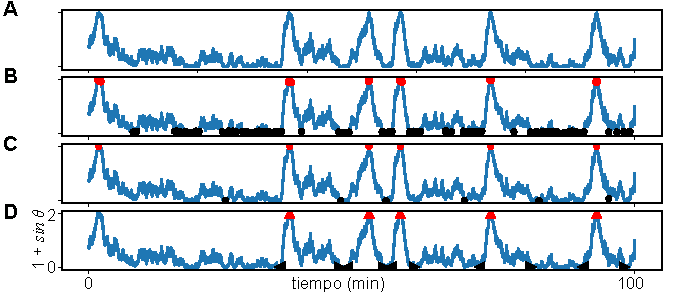
\includegraphics[width=1\columnwidth]{figures/chapter6/C6_pulse_detection.pdf} 
    \caption{\textbf{Algoritmo de detección de pulsos.} (A) Serie temporal sintética. (B) Paso intermedio del algoritmo de detección de pulsos, donde los máximos (rojo) y mínimos (negro) relativos que cumplen las condiciones umbrales están indicados. (C)  Paso intermedio del algoritmo de detección de pulsos, donde los máximos (rojo) y mínimos (negro) relativos filtrados están indicados. Con este filtro, se cumple entre dos máximos locales hay un sólo mínimo, y que entre dos mínimos locales hay un máximo. Estos son los puntos de referencia a partir de donde buscaremos el comienzo y el final de cada pulso. (D) Resultado del algoritmo de detección de pulsos, donde el inicio (triángulo negro con el vértice del lado izquierdo), el pico (rojo) y el final (triángulo negro con el vértice del lado derecho) están indicados. Parámetros: $\omega = \frac{2\pi}{7 \text{ min }}$, $\alpha = 1.01 \times \frac{2\pi}{7 \text{ min }}$, $ D = 0.1 \frac{1}{\text{min}^2}$. La tasa de adquisición fue de dt = 0.001, cada d = 1 pasos. El umbral de amplitud del algoritmo de detección de pulsos fue $A_{th} = 0.9$, y la distancia umbral fue de $W_{th} = 100\text{ cuadros}$.} 
    \label{C6_fig:pulse_detection}
\end{figure}
 

Continuamos por imponer que entre dos máximos locales haya un sólo mínimo, y que entre dos mínimos locales haya un máximo. Primero removemos todos los mínimos locales detectados antes del primer máximo local. Luego recorremos todos los pares de máximos locales sucesivos que detectamos. Empezamos por el primero y el segundo, continuamos por el segundo y el tercero, y así sucesivamente. 


Para cada par de máximos locales consecutivos, tomamos todos los mínimos locales que hayamos detectado entre ellos. Luego, removemos, de a uno, el mayor de este subgrupo de mínimos locales detectados, hasta tener uno sólo mínimo local. Si este subgrupo estaba inicialmente vacío, removemos el máximo menor del par de máximos locales que consideramos, y comenzamos otra vez redefiniendo el par de máximos sucesivos. Una vez recorridos todos los pares de máximos locales, removemos todos los mínimos detectados después del último máximo, a excepción de el primero. Con este procedimiento, logramos tener la misma cantidad de máximos y mínimos locales. Los máximos y mínimos locales funcionan como puntos de referencia a partir de donde buscaremos el comienzo y el final de cada pulso. A los máximos de referencia los llamaremos $M$, y a los mínimos de referencia $m$. La cantidad de los máximos de referencia $M$ es la misma que la de los mínimos de referencia $m$. Entonces, decimos que cada máximo $M_k$ tiene asociado un mínimo de referencia inmediatamente anterior $m_{k-1}$, y uno inmediatamente posterior $m_{k}$, a excepción del primer máximo $M_0$. El resultado de este paso intermedio se encuentra representado en la figura \ref{C6_fig:pulse_detection}C.


Los máximos de referencia $M$ se corresponden con un máximo en $X = \sin{\xx}$, es decir, en $\xx \approx \frac{\pi}{2} + 2n\pi$. Los mínimos de referencia $m$ se corresponden con un mínimo en $X = \sin{\xx}$, es decir, en $\xx \approx \frac{3\pi}{2} + 2n\pi$. Entonces, si nos paramos sobre un máximo $M_k$ y recorremos la fase en dirección contraria al tiempo hacia su mínimo inmediatamente anterior $m_{k-1}$, atravesaremos un punto fijo inestable. En cambio, si nos paramos sobre un máximo $M_k$ y recorremos la fase en la dirección del tiempo hacia su mínimo inmediatamente posterior $m_{k}$ , atravesaremos el punto fijo estable. Con esta idea buscaremos el principio y el final de los pulsos. 



Para cada máximo de referencia $M_k$, calculamos su número de vueltas completas $n$ que tiene la fase en ese instante, y se lo restamos momentáneamente a la variable angular $\xx' = \xx - 2n \pi$. Con esta transformación, $M_k$ queda posicionado entre el primer y segundo cuadrante, $m_{k-1}$ entre los cuadrantes $-1$ y $-2$, y $m_{k+1}$ entre los cuadrantes $3$ y $4$. Además, \xxe queda posicionado en el cuadrante $-1$, y \xxi en el cuadrante $3$. 


Recorremos la fase $\xx'$ desde el máximo $M_k$ en dirección contraria al tiempo hacia el mínimo inmediatamente anterior $m_{k-1}$. En esta dirección, esperamos que la fase \xx decrezca. En el caso del primer máximo, el final del recorrido es comienzo de la serie temporal. Cuando $\xx' - \xxe' \geq 0$, encontramos el punto fijo estable $C_k$, que consideramos el comienzo de un pulso. Puede ocurrir que no nos topemos con un punto fijo estable durante este recorrido. Por ejemplo, puede suceder con altos valores de ruido la fase crezca en dirección contraria al tiempo y no atraviese un punto fijo inestable. En estos casos, descartamos $M_k$ y su mínimo inmediatamente posterior $m_k$. Otro ejemplo es que en el caso oscilatorio puede que no encontremos al comienzo del pulso durante este recorrido, pues esperamos que el comienzo del pulso tenga una fase muy parecida al mínimo $m_{k-1}$. En ese caso, continuamos recorriendo la fase hasta el máximo $M_{k-1}$ inmediatamente anterior a $M_k$. En caso de no encontrar el punto fijo durante este recorrido, descartamos $M_k$ y su mínimo inmediatamente posterior $m_k$. Realizamos un procedimiento análogo para encontrar el punto fijo inestable $F_k$, es decir, el final de cada pulso, en este caso recorriendo la fase $\xx'$ desde $M_k$ hacia su mínimo inmediatamente posterior $m_k$.


Como resultado de este procedimiento, tendremos un conjunto de puntos fijos inestables $C$ que marcan el comienzo de los pulsos, un conjunto de máximos $M$ que señalizan el pico de un pulso, y un conjunto de puntos fijos estables $F$ que representan el final de los pulsos (figura \ref{C6_fig:pulse_detection}D). Con estos resultados, calculamos la duración de cada pulso $k$ como el tiempo que transcurre entre el principio $C_k$ y el final $F_k$ del pulso, y la tasa de pulsado como la cantidad de pulsos detectados en cada serie temporal $l$ sobre la duración de la serie temporal $T_l$, es decir, $\frac{\sum_k M_k}{T_l}$, donde $M_k$ es el pico del pulso $k$ de la serie temporal $l$. 


\marginpar{cálculo del intervalo\\de interpulsado}
Para calcular el intervalo de interpulsado, recorremos la serie temporal desde su inicio en dirección del tiempo. Para inicializar el procedimiento, anotamos el primer punto $Y_i$ cuya diferencia entre su fase y $\frac{3}{2}\pi$ sea mayor o igual que $2\pi$. Luego, continuado el recorrido, buscamos el primer punto $Y_f$ tal que la diferencia de fases entre $Y_1$ e $Y_0$ sea mayor o igual a $2\pi$. Una vez encontrado $Y_1$, el tiempo que transcurre entre $Y_f$ e $Y_i$ va a ser la primera medición de intervalo de interpulsado. Luego, repetimos el procedimiento  con $Y_f \rightarrow Y_i$ hasta terminar la serie temporal. Las mediciones realizadas con este método mostraban una estadística muy similar, pero un poco menos ruidosa, a calcular el intervalo de interpulsado como la diferencia temporal entre los picos de dos pulsos sucesivos, identificados a partir del algoritmo de detección de pulsos.  


\subsection{Comportamiento de los observables en el modelo teórico}

Buscamos entender si es posible ajustar los parámetros del modelo a los datos experimentales a partir de reproducir la estadística experimental de los observables que elegimos. Primero nos proponemos comprender cómo depende cada uno de estos observables de cada uno de los tres parámetros del modelo de fase con bifurcación de ciclo infinito y ruido blanco gaussiano aditivo. Luego, determinar si existe alguna región de parámetros en donde la estadística de los observables calculados sobre datos simulados es compatible con la observaciones sobre los datos experimentales, para dar lugar a una posible calibración. 

Exploramos la mediana de la distribución de duración de pulsos medida sobre las series temporales sintéticas de la fase en una grilla bidimensional de parámetros (figura \ref{C6_fig:2d_plots}A). Para comprender este gráfico, es útil enfocarse en el caso determinista representado por la línea vertical $D=0$, donde sólo varía la amplitud de modulación. Por ejemplo, cuando $\omega = \frac{2\pi}{7\; \text{min}}$, es posible ver que a medida que aumenta la amplitud de modulación desde cero hasta el valor de $\omega$ (linea negra punteada), la duración de pulsos aumenta. Esto es coherente con nuestra caracterización previa, donde observamos que los aumentos en la amplitud de modulación en el modelo determinista conducen a oscilaciones no uniformes. A medida que las oscilaciones son cada vez menos uniformes, su frecuencia disminuye y, en consecuencia, aumenta de la duración de pulsos (capítulo \ref{ch4}). Cuando $\alpha$ supera el valor de $\omega$, no se detectan pulsos en el régimen excitable, pues $D=0$ y no hay perturbaciones que puedan desencadenar actividad pulsátil. Si, en cambio, nos enfocamos en la línea horizontal donde $\alpha=0$, estaremos evaluando el caso de oscilaciones uniformes con ruido blanco gaussiano aditivo. En este caso, vemos que la duración de pulsos disminuye de izquierda a derecha conforme aumenta y domina el ruido por sobre el sistema dinámico.  


Con esta idea, observamos  en la figura \ref{C6_fig:2d_plots}A que, para una dada frecuencia del uniforme, en el régimen excitable la duración de pulsos disminuye en sentido diagonal, desde abajo a la izquierda hacia arriba a la derecha. Es decir, disminuye conforme aumentan ambas variables, la amplitud de modulación y la intensidad del ruido, comportamiento que observamos previamente para la duración de pulsos media (sección \ref{C6_sec:duracion}, figura \ref{C6_fig:duration}). Además, los valores de la duración de pulsos disminuyen conforme aumenta la frecuencia del uniforme, como también observamos previamente. En el régimen oscilatorio, la duración de pulsos disminuye cuando aumenta la intensidad del ruido y disminuye la amplitud de modulación, en sentido diagonal opuesto al caso del excitable. 

 \begin{figure}
    \centering 
    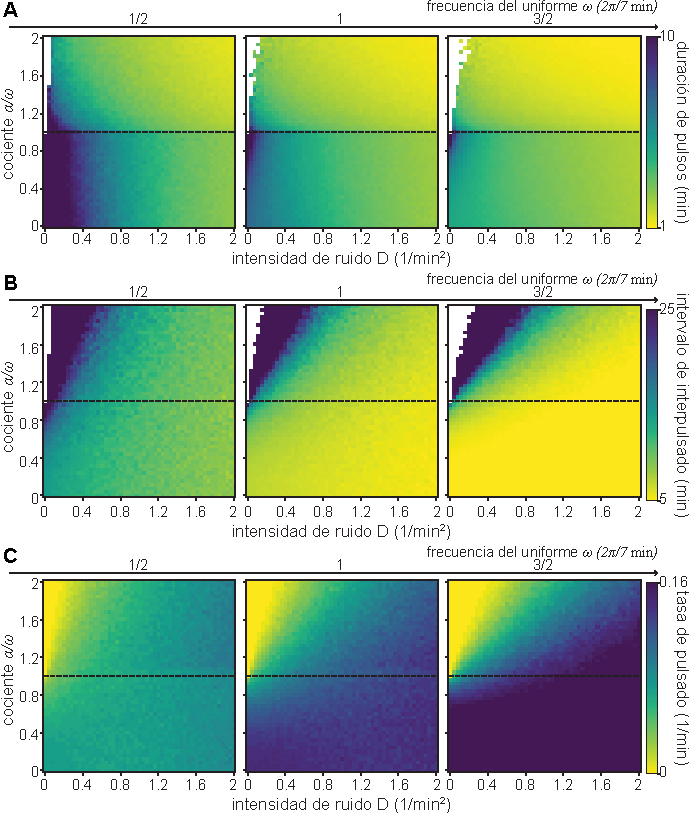
\includegraphics[width=1\columnwidth]{figures/chapter6/C6_2d_plots.pdf} 
    \caption{\textbf{Comportamiento de los observables elegidos en función de los parámetros del modelo}. Mediciones numéricas de la mediana de (A) la duración de pulsos, (B) el intervalo de interpulsado y (C) la tasa de pulsado en función de los parámetros del modelo. (A-C) Se observa el comportamiento en función de la intensidad del ruido $D$  y la amplitud de modulación $\alpha$. En cada caso, la frecuencia del uniforme es fija y su valor está indicado en la parte superior de cada gráfico. Los sectores blancos indican regiones donde no había actividad pulsátil en los datos simulados. La linea punteada negra indica el punto de bifurcación que separa el régimen oscilatorio (abajo) del excitable (arriba). La resolución de la amplitud de modulación es $0.04\; \frac{1}{\text{min}}$, y de la intensidad de ruido es $0.04\; \frac{1}{\text{min}^2}$. Cada punto de cada gráfico representa la adquisición de el observable correspondiente sobre una serie temporal de $T = 10000$ minutos de duración. La tasa de adquisición fue de $dt = 0.0001$, cada $d = 10$ pasos. El umbral de amplitud del algoritmo de detección de pulsos fue $A_{th} = 0.9$, y la distancia umbral fue de $W_{th} = 100 $ cuadros.}
    \label{C6_fig:2d_plots}
\end{figure}


La mediana de la distribución de intervalo de interpulsado medida sobre las series temporales sintéticas de la fase se encuentra representada en la figura \ref{C6_fig:2d_plots}B. Para una misma frecuencia del uniforme, este observable disminuye conforme aumenta la intensidad del ruido y disminuye la amplitud de modulación en ambos regímenes dinámicos. A diferencia de la duración de pulsos, en este caso no parece haber una discontinuidad o diferencia de comportamiento en la transición entre los regímenes dinámicos oscilatorio y excitable. Los valores de intervalo de interpulsado disminuyen conforme aumenta la frecuencia del uniforme. Finalmente, en la figura \ref{C6_fig:2d_plots}C observamos que la tasa de pulsado presenta un comportamiento opuesto a la distribución de intervalos de interpulsado. En este caso, la tasa de pulsado aumenta conforme aumenta la intensidad del ruido, disminuye la amplitud de modulación tanto en el régimen excitable como en el oscilatorio, y sus valores aumentan con la frecuencia del uniforme. Aunque sean opuestos, los comportamientos de ambos observables tiene origen en que la actividad pulsátil aumenta en esa dirección. Este aumento de actividad resulta en intervalos de interpulsado más cortos y tasas de pulsado más grandes. 


Para estudiar la compatibilidad de estas tres medidas con los valores adquiridos experimentalmente, primero identificamos en qué regiones de los mapas bidimensionales los valores de las medianas de cada observable estaban incluidos dentro de los rangos intercuartílicos de las distribuciones experimentales de la figura \ref{C6_fig:observables_experimentales}. En la figura \ref{C6_fig:2d_plots_sup}A coloreamos en negro los valores de la mediana de la duración de pulsos, el intervalo de interpulsado y la tasa de pulsado medidas a partir de las series temporales sintéticas si estos se encontraban en el intervalo definido entre el primer (Q25) y tercer cuartil (Q75) de las correspondientes distribuciones experimentales. Para todos los casos vemos que el área de la zona de coincidencia disminuye conforme aumenta la frecuencia del uniforme. Para la duración de pulsos, la superposición es más grande se da en el régimen oscilatorio. En cambio, para la distribución de interpulsado la mayor superposición ocurre en el excitable. Esto posiblemente sea consecuencia de que en los experimentos los pulsos tienen una duración definida, pero no siempre están organizados uno detrás de otro. Probablemente, esta sea también la razón de que la tasa de pulsado presente mayores áreas de superposición en el régimen excitable. 


Consideramos regiones de parámetros compatibles con los experimentos donde había superposición en los tres observables simultáneamente. En la figura \ref{C6_fig:2d_plots_sup}B observamos que existen regiones de parámetros en donde la estadística del modelo ajusta a las observaciones experimentales. En todos los casos, las regiones de compatibilidad se encontraban cerca de la zona de bifurcación. Además, vimos que esta compatibilidad se reduce conforme aumenta la frecuencia del oscilatorio. Posiblemente si continuamos reduciendo $\omega$, encontremos más regiones de parámetros en donde el modelo es compatible con el experimento. 


Este procedimiento manual en donde estudiamos la compatibilidad entre el modelo y los experimentos nos informa que existen regiones del espacio de parámetros del modelo teórico considerado que reproducen los estadísticos medidos sobre los experimentos. Este procedimiento se vuelve poco práctico para conseguir un ajuste de estos parámetros, y decidimos establecer un protocolo para ajustar de manera sistemática los parámetros del modelo, que describimos a continuación. 



 \begin{figure}
    \centering
    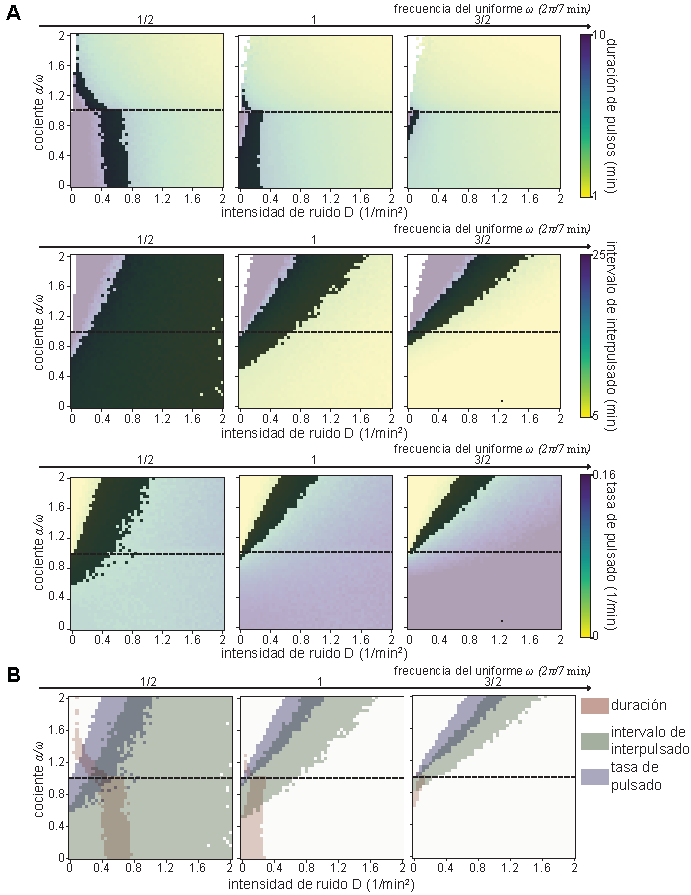
\includegraphics[width=1\columnwidth]{figures/chapter6/C6_2d_plots_superposition.pdf} 
    \caption{\textbf{Superposición de los observables elegidos en función de los parámetros del modelo}. (A) Mediciones numéricas de la mediana de la duración de pulsos, el intervalo de interpulsado y la tasa de pulsado en función de los parámetros del modelo. En cada gráfico, se observa el comportamiento en función de la intensidad del ruido $D$ y la amplitud de modulación $\alpha$. En cada caso, la frecuencia del uniforme es fija y su valor está indicado en la parte superior de cada gráfico. Los sectores negros indican las regiones donde los valores de las medianas adquiridas en el modelo teórico se encuentran dentro del rango intercuartilico de cada observable, definido como el intervalo entre el primer (Q25) y tercer (Q75) cuartil. Los sectores blancos indican regiones donde no había actividad pulsátil en los datos simulados. Cada punto de cada gráfico representa la adquisición de el observable correspondiente sobre una serie temporal de $T = 10000$ minutos de duración. La tasa de adquisición fue de $dt$ = $0.0001$, cada $d = 10$ pasos. El umbral de amplitud del algoritmo de detección de pulsos fue $A_{th} = 0.9$, y la distancia umbral fue de $W_{th} = 100\text{ cuadros}$. (B) Superposición de las regiones coloreadas en negro en A. En este caso, el sector blanco indica ausencia de superposición entre algún observable del modelo teórico y el experimento. (A,B) La linea punteada negra marca el punto de bifurcación que separa el régimen oscilatorio (abajo) del excitable (arriba). La resolución de la amplitud de modulación es $0.04\; \frac{1}{\text{min}}$, y de la intensidad de ruido es $0.04\; \frac{1}{\text{min}^2}$.}
    \label{C6_fig:2d_plots_sup}
\end{figure}





\subsection{Ajuste de las medidas experimentales}

Motivados por las superposiciones entre las estadísticas del modelo teórico que proponemos y los datos experimentales que adquirimos, buscamos establecer un protocolo para ajustar de manera sistemática la estadística de duración de pulsos, intervalo de interpulsado y tasa de pulsado observada en las mediciones experimentales de la dinámica de actividad de ERK en ESCs (figura \ref{C6_fig:observables_experimentales}). Implementamos el método de Cálculo Bayesiano Aproximado (ABC) basado en la implementación de Monte Carlo Secuencial (SMC) para obtener una distribución de probabilidad de los posibles $(\omega,\frac{\alpha}{\omega},D)$ que ajusten a nuestros datos experimentales.


\subsubsection{Implementación del Cálculo Bayesiano Aproximado Monte Carlo Secuencial}
\subsubsectionmark{Implementación del ABC-SMC}
\label{C6_sssec:implementac_ABCSMC}


%qué es el ABCMC
\marginpar{Cálculo Bayesiano\\Aproximado Monte\\Carlo Secuencial}
El método ABC-SMC busca inferir una distribución de probabilidad \textit{posterior} conjunta para los parámetros del modelo $(\omega,\frac{\alpha}{\omega},D)$, dada una distribución de probabilidad \textit{prior} que elegimos previamente para cada uno de los parámetros individuales \cite{Toni2009}. Como punto de partida, definimos la \textit{prior} a partir de nuestro conocimiento previo del modelo en función de qué parámetros consideramos razonables para describir los datos experimentales. La \textit{posterior} nos dirá cuál es la probabilidad de que nuestros datos provengan de un dado conjunto de parámetros $(\omega,\frac{\alpha}{\omega},D)$, dadas las mediciones experimentales.



% por qué elejimos el ABCMC
Por lo general, los métodos estadísticos bayesianos buscan obtener la \textit{posterior} a partir de la función de verosimilitud, una función de los parámetros del modelo teórico que es normalmente compleja. La ventaja del método ABC es que evita evaluar las funciones de verosimilitud y utiliza, en su lugar, métricas que se calculan a partir de simulaciones numéricas \cite{Csillery2010}. Está demostrado que, si el usuario elige las herramientas correctas a la hora de implementarlo, este método converge a la distribución \textit{posterior} \cite{Csillery2010,Filippi2013}. Por otro lado, SMC es una técnica paralelizable y particularmente eficiente para recorrer el espacio de parámetros durante la implementación del ABC. En este trabajo utilizamos la implementación de pyABC, disponible para python \cite{Klinger2018}.

%cómo lo implementamos 
Previo a la inicialización, definimos las \textit{prior} de cada uno de los parámetros $\omega,\frac{\alpha}{\omega},D$ como distribuciones uniformes dentro de intervalos que consideramos razonables luego de una inspección manual previa \cite{Toni2010} (ver apéndice \ref{C6_ap:ABC-SMC}). Para inicializar el método, se generan una serie de series temporales sintéticas a partir de $1000$ puntos tridimensionales $(\omega,\frac{\alpha}{\omega},D)$ muestreados del espacio de parámetros definido por las \textit{prior}. Se calcula la distancia $d$ de cada serie temporal sintética con los datos experimentales. En este trabajo, la mediana de estas distancias define la tolerancia $\epsilon$ que tendrá la primera iteración del algoritmo, y el peso (probabilidad estimada) de cada uno de las mil muestras del espacio de parámetros es inicialmente $w = \frac{1}{1000}$. 


En cada iteración, se elige un parámetro tridimensional $(\omega,\frac{\alpha}{\omega},D)$ de los $1000$ aceptados previamente. Esta elección se realiza en función de los pesos $w$ asociados a cada uno de los parámetros aceptados previamente. Luego, se perturba el parámetro tridimensional buscando obtener uno nuevo \cite{Toni2009}. La manera en se realiza esta perturbación influye en la eficiencia del algoritmo, pero no en su convergencia \cite{Filippi2013}. En este trabajo elegimos realizarla con un kernel gaussiano multivariado, y perturbamos cada conjunto de parámetros aceptados según una distribución normal multivariada con una matriz de covarianza que depende de la covarianza de la población aceptada anteriormente.

\begin{figure}
    \centering
    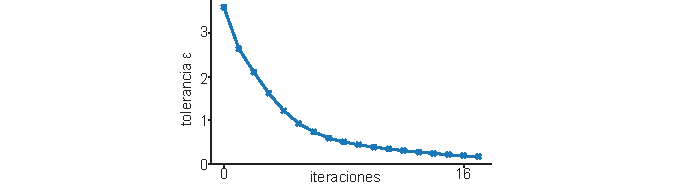
\includegraphics[width=1\columnwidth]{figures/chapter6/C6_eps.pdf} 
    \caption{\textbf{Convergencia del  Cálculo Bayesiano Aproximado Monte Carlo Secuencial}. Evolución de la tolerancia a medida que aumentan las iteraciones.}
    \label{C6_fig:eps}
\end{figure} 


A partir del nuevo parámetro que surge de esta perturbación, se simula una serie temporal larga y se calcula su distancia $d$ a los datos experimentales (ver apéndice \ref{C6_ap:ABC-SMC}). Este nuevo conjunto de parámetros será aceptado si la distancia entre los datos simulados y los experimentales es menor la tolerancia $\epsilon$ (figura \ref{C6_fig:eps}). Estas iteraciones se realizan hasta lograr aceptar nuevos $1000$ puntos tridimensionales del espacio de parámetros. 


Una vez aceptados nuevos $1000$ puntos, se actualiza las distribución de probabilidad de los parámetros y la tolerancia $\epsilon$. Las distribuciones de los parámetros se actualizan calculando nuevos pesos $w$ de los parámetros aceptados, y aquí también utilizamos el kernel gaussiano multivariado \cite{Toni2009}. Elegimos calcular la nueva tolerancia $\epsilon$ como la mediana de las distancias de la última población de parámetros aceptada. 


Evaluamos la convergencia del método siguiendo el valor de la tolerancia, y establecimos una tolerancia mínima que determinaba el final del algoritmo \cite{Costa2021} (figura \ref{C6_fig:eps}, ver apéndice \ref{C6_ap:ABC-SMC}). El valor de la tolerancia mínima refleja la tensión entre el costo computacional y la precisión del método. Si la tolerancia mínima es suficientemente chica, la distribución \textit{posterior} obtenida será una buena aproximación de la \emph{real} \cite{Toni2010}. El resultado es una muestra de $1000$ valores de parámetros a partir de la cual se infiere su distribución \textit{posterior} a través de sus pesos $w$ (ver apéndice \ref{C6_ap:ABC-SMC}). En definitiva, utilizamos una muestra finita de datos para hacer inferencias sobre la función de densidad de probabilidad subyacente en todo el espacio de parámetros. Los kernels gaussianos multivariados que utilizamos en este trabajo para realizar esta inferencia son una técnica no paramétrica para estimar estas funciones de densidad de probabilidad, considerada una generalización de estimar una distribución de probabilidad a partir de histogramas. 


Dados que los observables elegidos fueron la duración de pulsos, el intervalo de interpulsado y la tasa de pulsado, definimos la distancia entre los datos experimentales y los simulados como
\begin{equation}
    d = \sqrt{\frac{\sum_i (x_i - m_i)^2}{IQ_i^2}},
    \label{C6_eq:distancia_MC}
\end{equation}
donde $x_i$ y $IQ_i$ corresponden a la mediana ,y a la diferencia entre el primer y tercer cuartil (o rango intercuartílico) de cada uno de los observables $i$ sobre los datos experimentales, y $m_i$ es la mediana de cada uno de los observables $i$ sobre los datos sintéticos. Con esta definición, las simulaciones están cerca de los datos experimentales si la mediana de las distribuciones de los observables calculados a partir de las simulaciones se encuentran en el rango intercuartílico de las distribuciones experimentales. Más detalles técnicos sobre nuestra implementación se pueden encontrar en el apéndice \ref{C6_ap:ABC-SMC}.

\begin{figure}
    \centering
    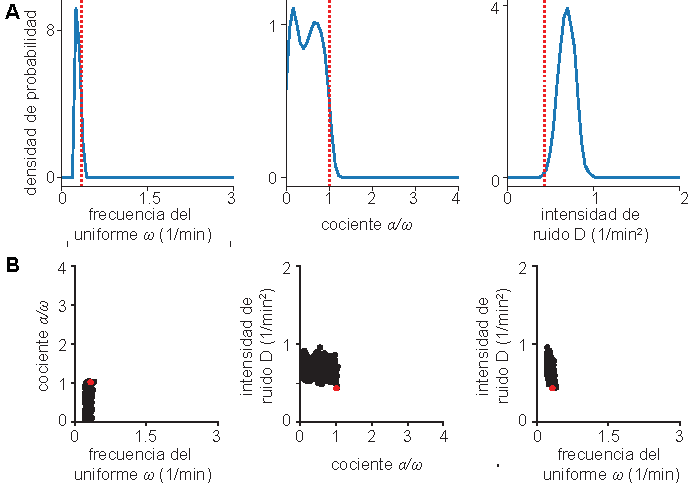
\includegraphics[width=1\columnwidth]{figures/chapter6/C6_fit_refval.pdf} 
    \caption{\textbf{\textit{Posterior} obtenida a partir del Cálculo Bayesiano Aproximado Monte Carlo Secuencial}. (A) Distribuciones marginales. La linea roja punteada indica el parámetro elegido para evaluar el ajuste. (B) Distribuciones marginales combinadas. El punto rojo indica el parámetro elegido para evaluar el ajuste. (A,B) Las distribuciones fueron obtenidas de la \textit{posterior} de los parámetros del modelo de fase de bifurcación de ciclo infinito y ruido blanco gaussiano aditivo de la ecuación \ref{C6_eq:adler_white_noise} que ajustan a los datos experimentales (figura \ref{C6_fig:observables_experimentales}). Decidimos graficar sólamente valores de $\frac{\alpha}{\omega} \geq 0$ porque en este trabajo decidimos restringir nuestro análisis sólo en valores positivos de los parámetros del modelo teórico. Parámetro elegido para evaluar el ajuste: $\omega = 0.333248630596246\;\frac{1}{\text{ min }}$, $\alpha = 1.01512115243615 \times \omega$, $ D = 0.431750499131804 \; \frac{1}{\text{min}^2}$ (ver apéndice \ref{C6_ap:ABC-SMC}).}
    \label{C6_fig:fit}
\end{figure} 



Como resultado, en la figura \ref{C6_fig:fit}A se encuentran las distribuciones marginales de la \textit{posterior} que surge de implementar este algoritmo. Las distribuciones marginales de la frecuencia del uniforme y de la intensidad del ruido resultaron ser unimodales y 
angostas, sugiriendo la existencia de un rango de valores que ajustan a los datos experimentales. Por otro lado, la distribución marginal del cociente \xx asociado a la amplitud de modulación era bimodal, con un máximo en valores pequeños y otro cercanos a $1$, siendo que la mayoría de los parámetros capaz de reproducir las métricas experimentales perteneces al régimen oscilatorio. Esto es coherente con que la moda de la distribución de frecuencias resultó ser menor que las contempladas para estudiar la compatibilidad del modelo con las observaciones experimentales de la figura \ref{C6_fig:2d_plots_sup}. Contemplando la distribución \textit{posterior} tridimensional, muchos de los parámetros más probables eran cercanos o mayores que uno (apéndice \ref{C6_ap:ABC-SMC}).  


En la figura \ref{C6_fig:fit}B observamos que los pares de distribuciones marginales de cada parámetro son una linea casi recta, vertical (paralela al eje $y$) u horizontal (paralela al eje $x$). A partir de estas observaciones, inferimos que los posibles valores de cada uno de los parámetros no tienen una correlación aparente. 


\subsubsection{Evaluación de los parámetros seleccionados}
\label{C6_sssec:evaluac_params}

A partir de la implementación del método ABC-SMC logramos estimar la función \textit{posterior}, que nos informa la probabilidad de que nuestras observaciones provengan de un dado conjunto de parámetros $(\omega,\ddelta,D)$, dadas la estadística de duración de pulsos, intervalo de interpulsado y tasa de pulsado. Esta distribución de probabilidad se infiere a partir de una muestra de $1000$ valores de parámetros a través de sus pesos $w$ (ver apéndice \ref{C6_ap:ABC-SMC}). 


Para continuar, queremos determinar la capacidad de este ajuste de reproducir los estadísticos que utilizamos en el capítulo \ref{ch2} para definir las oscilaciones intermitentes, como hicimos en la sección \ref{C2_sec:pulsado_estoctastico}. Estos estadísticos son (i) la cantidad de pulsos aislados y consecutivos, (ii) la actividad, y (iii) la frecuencia de trenes de pulsos de determinada longitud. Para realizar esta evaluación, calculamos estos tres estadísticos sobre series temporales sintéticas, y comparamos el resultado con las mediciones sobre los datos experimentales. Como el algoritmo de detección de pulsos para las simulaciones identifica el inicio, el pico y el final de cada pulso - al igual que la detección de pulsos implementada para los datos del capítulo \ref{ch2}- utilizamos las mismas estrategias que para los datos experimentales para realizar estos cálculos.


Para obtener estas series temporales sintéticas, elegimos uno de los $1000$ grupos de valores de parámetros $(\omega,\ddelta,D)$ que surgieron del ajuste ABC-SMC (en rojo en figura \ref{C6_fig:fit}). Elegimos utilizar un grupo de parámetros de alta probabilidad que ajuste a la cantidad total de pulsos que observamos en los experimentos. Con esta elección, es más sencillo comparar estos observables con otras mediciones realizadas sobre nuevos modelos teóricos. Para construir las figuras, realizamos simulaciones en donde la cantidad de trazas obtenidas era la misma que en los experimentos, y su duración similar (apéndice \ref{C6_ap:ABC-SMC}).


En la figura \ref{C6_fig:param_evaluation}A observamos la estadística sobre $100$ repeticiones de pulsos totales, aislados o consecutivos normalizados sobre la cantidad detectada en los experimentos. Con esta normalización, la recta $y = 1$ detallada en la figura remarca los valores experimentales. Observamos que si bien el modelo reproduce la cantidad de pulsos totales, sobrestima los aislados, y subestima los consecutivos. En la figura \ref{C6_fig:param_evaluation}B observamos que el modelo es capaz de reproducir la cantidad de trenes cortos de pulsos, pero subestima fuertemente la cantidad de trenes de más de $3$ pulsos de longitud. 


Además, observamos que, en promedio, tanto los datos sintéticos como los experimentales pulsaban la misma proporción de tiempo (derecha en figura \ref{C6_fig:param_evaluation}C). Evaluando el comportamiento poblacional, si bien el modelo ajusta correctamente los valores intermedios de actividad, fallan en reproducir los casos en los que las células únicas pulsaban casi todo el tiempo de medición o no pulsaban (izquierda en figura \ref{C6_fig:param_evaluation}B). La actividad poblacional es una medida sencilla que cuantifica la heterogeneidad dinámica característica de nuestras observaciones, característica que no fue posible reproducir con el modelo teórico propuesto.

\begin{figure}
    \centering
    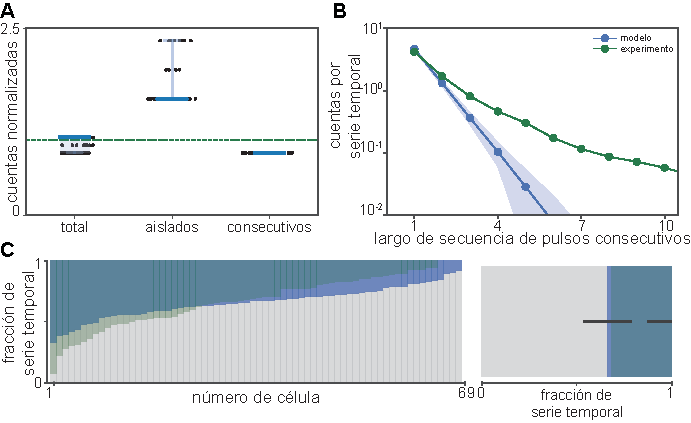
\includegraphics[width=1\columnwidth]{figures/chapter6/C6_param_evaluation.pdf} 
    \caption{\textbf{Capacidad del ajuste del ajuste del Cálculo Bayesiano Aproximado Monte Carlo Secuencial para reproducir los observables que describen las oscilaciones intermitentes.} (A)  Mediana de pulsos totales, consecutivos y aislados, normalizados por la mediana de los datos experimentales (puntos negros). Los datos provienen de 100 realizaciones del modelo teórico. Las barras de color representan la mediana, los límites de la caja son los percentiles 25 y 75 de las distribuciones, y los bigotes son los percentiles 5 y 95. La linea verde referencia los valores experimentales. (B) Número de trenes de pulsos en función del número de pulsos consecutivos en el tren para las simulaciones (naranja) y los datos experimentales (verde). El recuento incluye los casos que se producen dentro de trenes más largos, y el primer punto de datos corresponde al número total de pulsos individuales. Los recuentos se han normalizado por el número de series temporales. El área sombreada es desviación estándar de 100 realizaciones independientes del modelo teórico. (C) Izquierda: fracción de tiempo que las series temporales sintéticas individuales pasaron pulsando (naranja) o sin pulsar (gris). A la derecha: Tiempo medio que las series temporales estuvieron pulsando (naranja) o no pulsando (gris). La barra de error indica la desviación estándar calculada sobre la población celular. En verde se indican las mediciones realizadas sobre los experimentos realizados en serum + LIF (capítulo \ref{ch2}). Estas mediciones fueron calculadas sobre 69 series temporales sintéticas de 120 minutos de duración, un conjunto de datos similar al experimental. (A-C) Parámetros:  $\omega = 0.333248630596246\;\frac{1}{\text{ min }}$, $\alpha = 1.01512115243615 \times \omega$, $ D = 0.431750499131804 \; \frac{1}{\text{min}^2}$. La tasa de adquisición fue de $dt = 0.001$, cada $d = 1$ pasos. El umbral de amplitud del algoritmo de detección de pulsos fue $A_{th} = 0.9$, y la distancia umbral fue de $W_{th} = 100\text{ cuadros}$. N = $69$ series temporales. $T = 120$ minutos de duración (ver apéndice \ref{C6_ap:ABC-SMC},figura \ref{C6_ap_fig:traces_evaluation})}
    \label{C6_fig:param_evaluation}
\end{figure} 


Estas observaciones nos sugieren que, en el modelo teórico, los pulsos son aislados o se organizan en en trenes cortos. Que el modelo logre reproducir la cantidad de pulsos totales y la actividad media es a costa de sobrestimar la cantidad de pulsos aislados, y permitir que más series temporales tengan actividad pulsátil. Como en este modelo la actividad pulsátil tiende a ser más homogénea a lo lago de la población, esto conduce a fallar en reproducir la heterogeneidad de tiempo de pulsado que observamos en los experimentos. 


Por completitud, los histogramas de la estadística de duración de pulsos, intervalo de interpulsado y tasa de pulsado calculados a partir de las simulaciones analizadas en \ref{C6_fig:param_evaluation} se encuentran en la figura \ref{C6_fig:dist_param_evaluation_hist}. Si bien las medianas de las distribuciones simuladas se encuentran dentro de los intervalos intercuartílicos experimentales, su distancia no responde a los valores mínimos de tolerancia del ajuste ABC-SMC (ecuación \ref{C6_eq:distancia_MC}, apéndice \ref{C6_ap:ABC-SMC}). Esto es consecuencia de generar los histogramas a partir de simulaciones con las mismas características que los datos experimentales, lo que aporta cierta variabilidad a las medianas de estos histogramas. 



\begin{figure}
    \centering
    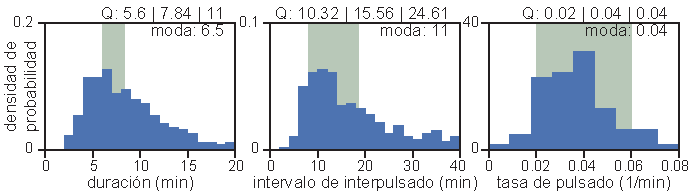
\includegraphics[width=1\columnwidth]{figures/chapter6/C6_param_evaluation_hist.pdf} 
    \caption{\textbf{Distribuciones de duración de pulsos, intervalo de interpulsado y tasa de pulsado del ajuste del Cálculo Bayesiano Aproximado Monte Carlo Secuencial}. Distribuciones de la duración de pulsos, el intervalo de interpulsado y la tasa de pulsado, calculadas sobre 69 series temporales sintéticas de 120 minutos de duración, un conjunto de datos similar al experimental. Las unidades del eje $y$ son (1/min), (1/min) y min respectivamente. N = 69 células, $n_1$ = 321 pulsos, $n_2$ = 252 pares de pulsos. Los cuartiles (Q) 25, 50 y 75 y la moda se indican en la parte superior de cada gráfico. Fueron excluidos de los histogramas 5 (duración) y 22 (intervalo de interpulsado) puntos mayores que el límite del eje x. En verde se indica el rango intercuartílico $IQ$ correspondiente a los experimentos realizados en serum + LIF (figura \ref{C6_fig:observables_experimentales}). Parámetros:  $\omega = 0.333248630596246\;\frac{1}{\text{ min }}$, $\alpha = 1.01512115243615 \times \omega$, $ D = 0.431750499131804 \; \frac{1}{\text{min}^2}$. La tasa de adquisición fue de $dt = 0.001$, cada $d = 1$ pasos. El umbral de amplitud del algoritmo de detección de pulsos fue $A_{th} = 0.9$, y la distancia umbral fue de $W_{th} = 100\text{ cuadros}$. N = $69$ series temporales. $T = 120$ minutos de duración (figura \ref{C7_fig:dist_traces_VM}).}
    \label{C6_fig:dist_param_evaluation_hist}
\end{figure} 



En el caso de la duración de pulsos, obtuvimos una distribución más ancha y asimétrica que la de los datos experimentales, con valores máximos de duración más grandes, pero con valores mínimos similares. En el caso de la distribución de intervalo de interpulsado, pudimos satisfactoriamente reproducir su asimetría característica, pero menos definida y con valores mayores. Esto probablemente sea consecuencia de subestimarla cantidad de pulsos consecutivos, responsables de los intervalos de interpulsado cortos. En el histograma de tasa de pulsado, observamos una baja proporción de series temporales sin pulsos y con muchos pulsos. Esta característica probablemente sea un reflejo tener una actividad pulsátil más homogénea que en los experimentos. 


Como conclusión, creemos que el modelo de fase con bifurcación de ciclo infinito y ruido blanco gaussiano es insuficiente para reproducir las oscilaciones intermitentes de actividad de ERK en ESCs. Esta descripción es incapaz de reproducir la estadística de trenes de pulsos largos, así como la heterogeneidad poblacional de la actividad pulsátil. Estos resultados sugieren que no es suficiente asumir que los pulsos son producto de excitaciones del régimen excitable, o actividad pulsátil oscilatoria cuya coherencia se destruye con el ruido blanco gaussiano. Motivados por estas observaciones, en el siguiente capítulo proponemos modificaciones al modelo teórico para intentar reproducir satisfactoriamente nuestras observaciones. 




\section{Conclusiones y discusión}

%Nuestra motivación es describir la dinámica de actividad de ERK en ESCs, donde intervalos oscilatorios se intercalan con intervalos de silencio y pulsos aislados. En el capítulo anterior vimos que la forma normal de un modelo de fase con bifurcación de ciclo infinito podría potencialmente describir a los pulsos aislados que observamos en los experimentos, pero en su versión determinista es insuficiente, pues carece de actividad pulsátil en el régimen excitable. En este capítulo proponemos perturbar de manera sistemática al modelo de fase con bifurcación de ciclo infinito añadiendo al modelo ruido blanco gaussiano aditivo.


%Primero, estudiamos las propiedades de la forma normal del modelo de fase con bifurcación de ciclo infinito con ruido blanco gaussiano aditivo. En sistemas lejos del equilibrio, el ruido está presente inevitablemente, y sus orígenes pueden ser muy diversos \cite{Lindner2004}. En particular, el ruido puede estar presente en sistemas excitables como reacciones químicas, lásers, la dinámica del clima, neuronas, e incluso en redes de transducción de señales intracelulares como las que regulan la dinámica de ERK es ESCs. Cómo el ruido afecta a sistemas excitables es una pregunta relevante para muchas áreas del conocimiento, y presenta muchas aplicaciones. 


%En el régimen excitable, el ruido promueve las excursiones del sistema dinámico a lo largo de la circunferencia trigonométrica, que en el observable \ref{C5_eq:seno_fase} se traduce en actividad pulsátil (figura \ref{C6_fig:traces}). A partir del espectro de consenso de las series temporales del observable y el correspondiente factor de calidad, identificamos que existe un valor de intensidad del ruido que optimiza la coherencia de la actividad pulsátil en este régimen, efecto conocido como resonancia estocástica (figura \ref{C6_fig:SR}A,B). Esto sucede porque, contrariamente a nuestra intuición, ante determinadas circunstancias, el ruido puede mejorar el rendimiento de determinados procesos. Por ejemplo, la resonancia estocástica puede optimizar la transmisión de información \cite{Gammaitoni1998}. Por otro lado, en el régimen oscilatorio, observamos que las oscilaciones pierden su regularidad a medida que crece el ruido, y el ruido destruye la coherencia de las oscilaciones (figuras \ref{C6_fig:traces}, \ref{C6_fig:SR}C,D). 


%En el capítulo anterior observamos que la duración de pulsos en el régimen excitable es sensible a las perturbaciones que dan lugar a la actividad pulsátil. Motivados por este resultado, obtuvimos una expresión analítica para la duración de pulsos. Esta expresión nos permite estudiar su dependencia de los distintos parámetros del modelo, entre ellos el ruido. 

%Para realizar este cálculo, primero nos enfocamos en estudiar la probabilidad de que el sistema dinámico atraviese el punto fijo estable pero no el punto fijo inestable en función de su condición inicial, cálculo que extendimos también al caso oscilatorio (figura \ref{C6_fig:mFPT_eps}). Observamos que para valores chicos de ruido, siempre que el sistema empiece fuera del punto fijo inestable, inevitablemente termina en el punto fijo estable y no vuelve al punto fijo inestable. A medida que aumenta la intensidad del ruido, la probabilidad se va suavizando y el sistema se tiende a comportar como un \textit{random walk} simétrico, donde la dinámica está gobernada por el ruido. Luego calculamos el tiempo medio que tarda el sistema en realizar este recorrido, también en función de su condición inicial (figura \ref{C6_fig:mFPT_tplus}). Observamos que tanto el ruido, como la frecuencia de modulación y la frecuencia del uniforme, todos tienden a disminuir el tiempo requerido para realizar el recorrido. 


%Finalmente, logramos obtener una expresión analítica para el tiempo medio que tardaba el sistema en atravesar el punto fijo estable habiendo salido y no vuelto al punto fijo inestable, es decir, la duración media de un pulso (figura \ref{C6_fig:duration}). Este cálculo, previamente no reportado, lo hicimos extensivo al caso oscilatorio. Observamos que la duración de pulsos depende de los parámetros del modelo de una manera no trivial. 


%La duración de pulsos disminuye conforme aumenta el ruido, y para valores altos de intensidad de ruido, las curvas convergen a una duración límite finita que es independiente del resto de los parámetros del modelo. Por otro lado, observamos una discontinuidad en la duración de pulsos en función de \ddelta donde ocurre la bifurcación del modelo determinista ($\ddelta = 1$). Para el caso oscilatorio donde $\ddelta < 1$, si la duración de pulsos es creciente o decreciente con \ddelta depende de los parámetros $D$ y $\omega$, y, en particular, en la bifurcación aumenta con ambos parámetros. Es razonable hipotetizar que, para valores muy pequeños de ruido, la duración de pulsos en el régimen oscilatorio tienda a comportarse según \ref{C5_eq:T_osc}, y en el excitable según \ref{C5_eq:T_exc}, resultados que obtuvimos para el modelo determinista. En el régimen excitable donde $\ddelta > 1$, la duración de pulsos siempre decrece conforme aumenta \ddelta, como observamos en el capítulo anterior. Finalmente, observamos que para frecuencias del uniforme cada vez más altas, la duración de pulsos disminuye.  



En consiguiente, nos preguntamos cuáles eran las capacidades y limitaciones del modelo estocástico propuesto de reproducir nuestras observaciones experimentales de la dinámica de activación de ERK en ESCs. Comenzamos por evaluar su capacidad de ajustar a tres observables calculados sobre los datos experimentales: la duración de pulsos, el intervalo de interpulsado y la tasa de pulsado (figura \ref{C6_fig:observables_experimentales}). Para esto, primero desarrollamos métodos computacionales para medir estas cantidades en series temporales de la fase (figura \ref{C6_fig:pulse_detection}), y estudiamos la dependencia de estos observables de los parámetros del modelo teórico. 

Exploramos la mediana de la distribución de duración de pulsos medida sobre las series temporales sintéticas de la fase en una grilla bidimensional de parámetros (figura \ref{C6_fig:2d_plots}). Coherentemente con nuestro análisis previo, observamos que la duración de pulsos disminuye conforme aumenta la frecuencia del uniforme y la intensidad del ruido. En el régimen excitable disminuye conforme aumentan la amplitud de modulación, y en el oscilatorio cuando ésta disminuye. Por otro lado, observamos que el intervalo de interpulsado y la tasa de pulsado presentan dependencias complementarias.  Mientras que cuando aumenta la intensidad del ruido, disminuye la amplitud de modulación y aumenta la frecuencia del uniforme el intervalo de interpulsado disminuye, la tasa de pulsado aumenta. Los comportamientos de ambos observables tiene origen en que la actividad pulsátil aumenta en esa dirección. Este aumento de actividad resulta en intervalos de interpulsado más cortos y tasas de pulsado más grandes. Además, a diferencia de la duración de pulsos, en estos casos no parece haber una discontinuidad o diferencia de comportamiento en la transición entre los regímenes dinámicos oscilatorio y excitable. Asimismo, observamos que la estadística de estas tres medidas calculadas sobre el modelo teórico eran compatibles con los valores adquiridos experimentalmente, ya que identificamos regiones de los mapas bidimensionales los valores de las medianas de estos observables estaban incluidos dentro de los rangos intercuartílicos de las distribuciones experimentales simultáneamente (figura \ref{C6_fig:observables_experimentales}). 


Motivados por las superposiciones entre las estadísticas del modelo teórico que proponemos y los datos experimentales que adquirimos, quisimos conocer qué conjunto de parámetros del modelo teórico reproduce la estadística observada en las mediciones experimentales. Implementamos el método de Cálculo Bayesiano Aproximado basado en la implementación de Monte Carlo Secuencial para obtener una distribución de probabilidad \textit{posterior} de los posibles $(\omega,\frac{\alpha}{\omega},D)$ que ajusten a nuestros datos experimentales (figura  \ref{C6_fig:fit}). 


Las distribuciones marginales de la frecuencia del uniforme y de la intensidad del ruido resultaron ser unimodales y angostas, sugiriendo la existencia de un rango de valores que ajustan a los datos experimentales, y los pares de distribuciones marginales de cada parámetro mostraron que los posibles valores de cada uno de los tres parámetros del modelo no tenían una correlación aparente. Por otro lado, la distribución marginal del cociente \xx asociado a la amplitud de modulación era bimodal y con ambas modas menores a uno, y la mayoría de los parámetros capaz de reproducir las métricas experimentales pertenecían al régimen oscilatorio. Si bien en la distribución \textit{posterior} tridimensional muchos de los parámetros más probables eran cercanos o mayores que uno, esta característica de la distribución marginal del cociente \xx nos lleva a replantearnos la principal motivación para comenzar a trabajar con este modelo. La idea de perturbar de manera sistemática al sistema en el régimen excitable para reproducir las oscilaciones intermitentes no parece ser suficiente, e incluso las oscilaciones desordenadas por el ruido parecen ajustar mejor a nuestras mediciones experimentales (apéndice \ref{C6_ap:ABC-SMC}).  



Comparamos la estadística de los datos experimentales con la surgida de series sintéticas simuladas a partir de un conjunto de parámetros que obtuvimos como resultado de la implementación del ABC-SMC para determinar la capacidad de este ajuste de reproducir las oscilaciones intermitentes de actividad de ERK (figura \ref{C6_fig:param_evaluation}). Logramos reproducir la cantidad total de pulsos que observamos en el experimento, pero sobrestimando la cantidad total de pulsos aislados y subestimando la cantidad de consecutivos. Coherente con este resultado, el modelo fue capaz de reproducir la cantidad de trenes cortos de pulsos, pero subestima fuertemente la cantidad de trenes largos. Además, si bien el modelo reprodujo correctamente la proporción promedio que los datos experimentales pulsaban, los datos sintéticos fallaban en reproducir la heterogeneidad de actividad pulsátil que observamos en los datos experimentales. En particular, fallaban en reproducir los casos en los que las células individuales pulsaban durante toda la medición, o que no pulsaban nunca. 


Que existan regiones del espacio de parámetros del modelo teórico que puedan recapitular mediciones clave que realizamos sobre los datos experimentales presenta un panorama alentador para describir las oscilaciones intermitentes de actividad de ERK en ESCs. Sin embargo, que el modelo logre reproducir la cantidad de pulsos totales y la actividad media a costa de sobrestimar la cantidad de pulsos aislados presenta una limitación. Además, en el modelo teórico la mayoría de los pulsos son aislados o se organizan en en trenes cortos, característica que también se evidenció en una cola más larga en la distribución de intervalos de interpulsado de las simulaciones (figura \ref{C6_fig:dist_param_evaluation_hist}). Con esto, más series temporales presentan actividad pulsátil, conduciendo a una distribución de tasa de pulsado más definida que la experimental. Como en este modelo la actividad pulsátil tiende a ser más homogénea a lo lago de la población, esto conduce a fallar en reproducir la heterogeneidad de tiempo de pulsado. Con estas observaciones, creemos que el modelo de fase con bifurcación de ciclo infinito y ruido blanco gaussiano es insuficiente para reproducir las oscilaciones intermitentes de ERK en ESCs. Inspirados en estos resultados, en el próximo capítulo proponemos modificaciones al modelo teórico en vistas de dar con una descripción teórica de las oscilaciones intermitentes de actividad de ERK que observamos en ESCs.


\begin{comment}
%Sin embargo, nuestra interpretación es que el sistema dinámico de FGF/ERK se encuentra en el entorno de una bifurcación, y que variando el estímulo de FGF se promueve intervalos oscilatorios más largos, pero la duración de pulsos se conserva. 

Por otro lado, la dinámica que buscamos describir tiene una duración de pulsos fija.  Dado el carácter estocástico de las perturbaciones, esa sensibilidad podría contribuir a la variabilidad de la distribución de duración de pulsos que observamos en las series temporales de ERK. in embargo, desconocemos cómo depende la duración de pulsos en estos diversos contextos. 

%VER!!! OJO QUE LO DE ARRIBA TIENE IDEAS REPETIDAS CON LO DE ABAJO. tamnién en la seccioón posterior. quiero estudiar la dependencia del ruidoo de todos los parametros?
Los autores de \cite{Qian2000} proponen que quien determina la frecuencia máxima del espectro de frecuencias $\omega_0$ en el régimen excitable es el movimiento fuera de la \emph{cuenca} de atracción hacia el punto fijo estable. Según definimos en la sección \ref{C5_sec:T_exc}, el tiempo que el sistema pasa fuera de la cuenca de atracción hacia el punto fijo estable está íntimamente relacionado con la duración de los pulsos. Resulta, entonces, interesante, determinar cómo depende la duración de pulsos de la intensidad del ruido en este régimen. 

\end{comment}


\begin{subappendices}

\begin{comment}
ESTA FIGURA TIENE LOS PARAMS VIEJOS OJO
Las series temporales surgidas del conjunto de parámetros que elegimos para validar el modelo, así como el resultado del algoritmo de detección de pulsos se encuentran en la figura \ref{C6_ap_fig:traces_evaluation}. 

\begin{figure}
    \centering
    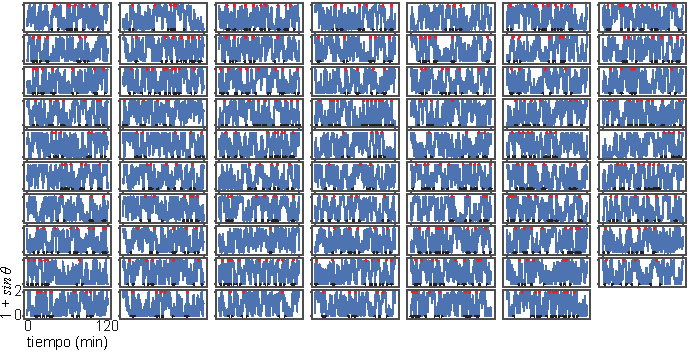
\includegraphics[width=1\columnwidth]{figures/chapter6/C6_ap_traces_for_evaluation.pdf} 
    \caption{\textbf{Series temporales sintéticas y detección de pulsos para validar el modelo teórico.} Series temporales del observable \ref{C5_eq:seno_fase} de la fase en función del tiempo. Se encuentra también representado el resultado del algoritmo de detección de pulsos, donde el inicio (triángulo negro con el vértice del lado izquierdo), el pico (rojo) y el final (triángulo negro con el vértice del lado derecho) de cada pulso detectado están indicados. Parámetros: $\omega = \frac{0.35887628760482}{\text{ min }}$, $\alpha = 0.646688055514436 \times \omega$, $ D = 0.774214789866716 \; \frac{1}{\text{min}^2}$. La tasa de adquisición fue de dt = 0.001, cada d = 1 pasos. El umbral de amplitud del algoritmo de detección de pulsos fue $A_{th} = 0.9$, y la distancia umbral fue de $W_{th} = 100\text{ cuadros}$. N = $69$ series temporales. $T = 120$ minutos de duración.}
    \label{C6_ap_fig:traces_evaluation}
\end{figure}
\end{comment}

\end{subappendices}
\end{document}